\documentclass[aspectratio=169,10pt]{beamer}

\usepackage[T1]{fontenc}
\usepackage{sourcesanspro}
\usepackage{sourcecodepro}
\usepackage{booktabs}
\usepackage{tabularx}
\usepackage{array}
\usepackage{graphicx}
\usepackage{tikz}
\usepackage{pgfplots}
\usepackage{fontawesome5}
\usetikzlibrary{arrows.meta,positioning,fit,calc,shapes.geometric}
\pgfplotsset{compat=1.18}

\definecolor{ArchInk}{HTML}{20252B}
\definecolor{ArchMuted}{HTML}{59636D}
\definecolor{ArchBlue}{HTML}{1F5F7A}
\definecolor{ArchBlueLight}{HTML}{EAF3F7}
\definecolor{ArchGreen}{HTML}{3D7A57}
\definecolor{ArchGreenLight}{HTML}{EDF6EF}
\definecolor{ArchRed}{HTML}{A42A38}
\definecolor{ArchRedLight}{HTML}{FAECEE}
\definecolor{ArchGold}{HTML}{B47A18}
\definecolor{ArchGoldLight}{HTML}{FBF3E3}
\definecolor{ArchLine}{HTML}{C8D1D8}
\definecolor{ArchPanel}{HTML}{F6F8F9}

\setbeamercolor{normal text}{fg=ArchInk,bg=white}
\setbeamercolor{structure}{fg=ArchBlue}
\setbeamercolor{frametitle}{fg=ArchInk,bg=white}
\setbeamercolor{alerted text}{fg=ArchRed}
\setbeamerfont{title}{size=\fontsize{26}{30}\selectfont,series=\bfseries}
\setbeamerfont{subtitle}{size=\fontsize{13}{16}\selectfont}
\setbeamerfont{frametitle}{size=\fontsize{18}{22}\selectfont,series=\bfseries}
\setbeamerfont{footline}{size=\fontsize{6.8}{8}\selectfont}
\setbeamertemplate{navigation symbols}{}
\setbeamertemplate{itemize item}{\color{ArchBlue}\small$\blacksquare$}
\setbeamertemplate{itemize subitem}{\color{ArchMuted}\scriptsize$\blacktriangleright$}
\setbeamersize{text margin left=0.55cm,text margin right=0.55cm}

\setbeamertemplate{frametitle}{%
  \nointerlineskip
  \begin{beamercolorbox}[wd=\paperwidth,ht=0.72cm,dp=0.13cm,leftskip=0.58cm,rightskip=0.58cm]{frametitle}
    \usebeamerfont{frametitle}\insertframetitle
  \end{beamercolorbox}
  \vspace{-0.08cm}
  \hspace{0.58cm}\color{ArchBlue}\rule{1.15cm}{0.75pt}\color{ArchLine}\rule{\dimexpr\paperwidth-2.31cm\relax}{0.35pt}
  \vspace{0.12cm}
}

\setbeamertemplate{footline}{%
  \leavevmode
  \hbox{%
    \begin{beamercolorbox}[wd=.72\paperwidth,ht=0.31cm,dp=0.12cm,leftskip=0.58cm]{footline}
      \color{ArchMuted}Architecture 2.0 \enspace|\enspace Principles for AI-Assisted System and Chip Design
    \end{beamercolorbox}%
    \begin{beamercolorbox}[wd=.28\paperwidth,ht=0.31cm,dp=0.12cm,rightskip=0.58cm plus 1fil]{footline}
      \hfill\color{ArchMuted}\insertframenumber
    \end{beamercolorbox}%
  }
}

\newcommand{\claim}[1]{%
  \begin{beamercolorbox}[rounded=true,sep=0.12cm,wd=\linewidth]{block body}
    \color{ArchBlue}\bfseries #1
  \end{beamercolorbox}\vspace{0.12cm}
}
\newcommand{\source}[1]{%
  \vfill{\fontsize{5.8}{7}\selectfont\color{ArchMuted}Source: #1\par}
}
\newcommand{\tagbox}[3]{%
  \begin{tikzpicture}[baseline=(n.base)]
    \node[rounded corners=2pt,fill=#1,draw=#2,inner xsep=5pt,inner ysep=3pt,
      text=ArchInk,font=\small\bfseries] (n) {#3};
  \end{tikzpicture}
}
\newcommand{\bigsep}[1]{%
  \begin{center}
    \begin{tikzpicture}
      \node[rounded corners=3pt,fill=ArchBlueLight,draw=ArchBlue,
        text width=13.2cm,align=center,minimum height=1.0cm,
        font=\fontsize{17}{20}\selectfont\bfseries,text=ArchBlue] {#1};
    \end{tikzpicture}
  \end{center}
}

\title{Architecture 2.0}
\subtitle{Principles for AI-Assisted System and Chip Design}
\author{Vijay Janapa Reddi}
\date{}

\begin{document}

% 1
\begin{frame}[plain]
  \begin{tikzpicture}[remember picture,overlay]
    \fill[ArchBlue] (current page.north west) rectangle ([xshift=0.14cm]current page.south west);
  \end{tikzpicture}
  \vspace{0.55cm}
  {\color{ArchMuted}\small SYNTHESIS LECTURE\par}
  \vspace{0.35cm}
  {\usebeamerfont{title}\color{ArchInk}\inserttitle\par}
  \vspace{0.12cm}
  {\usebeamerfont{subtitle}\color{ArchMuted}\insertsubtitle\par}
  \vspace{0.45cm}
  \begin{center}
    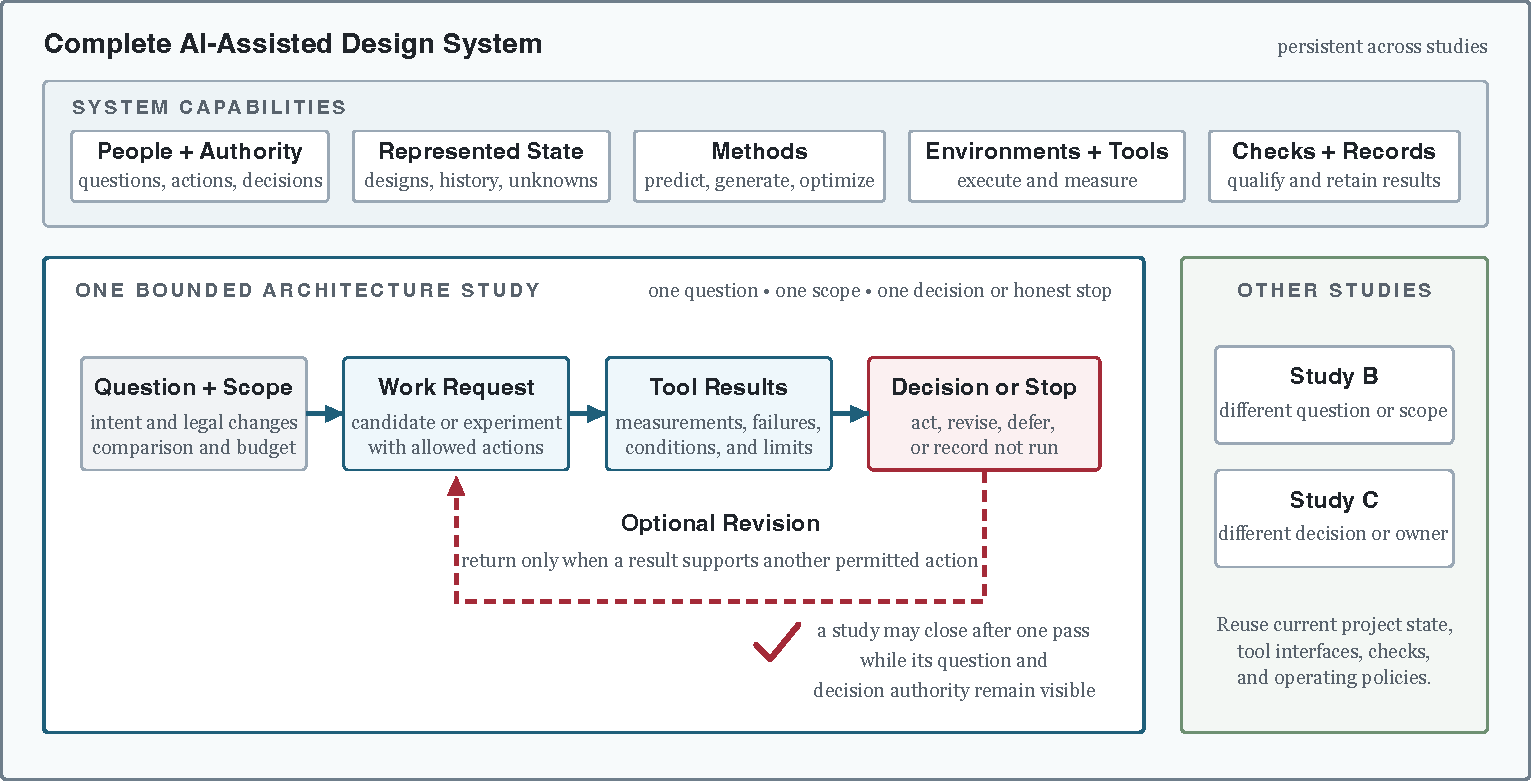
\includegraphics[width=0.72\linewidth,height=3.35cm,keepaspectratio]{../book/images/arch2-loop-diagram.pdf}
  \end{center}
  \vfill
  {\small\color{ArchInk}\insertauthor\hfill\color{ArchMuted}arch2.mlsysbook.ai\par}
\end{frame}

% 2
\begin{frame}{Three fields, one architecture decision}
  \claim{The useful intersection is not ``AI for chips.'' It is a supported architecture decision.}
  \begin{columns}[c,onlytextwidth]
    \column{0.58\textwidth}
      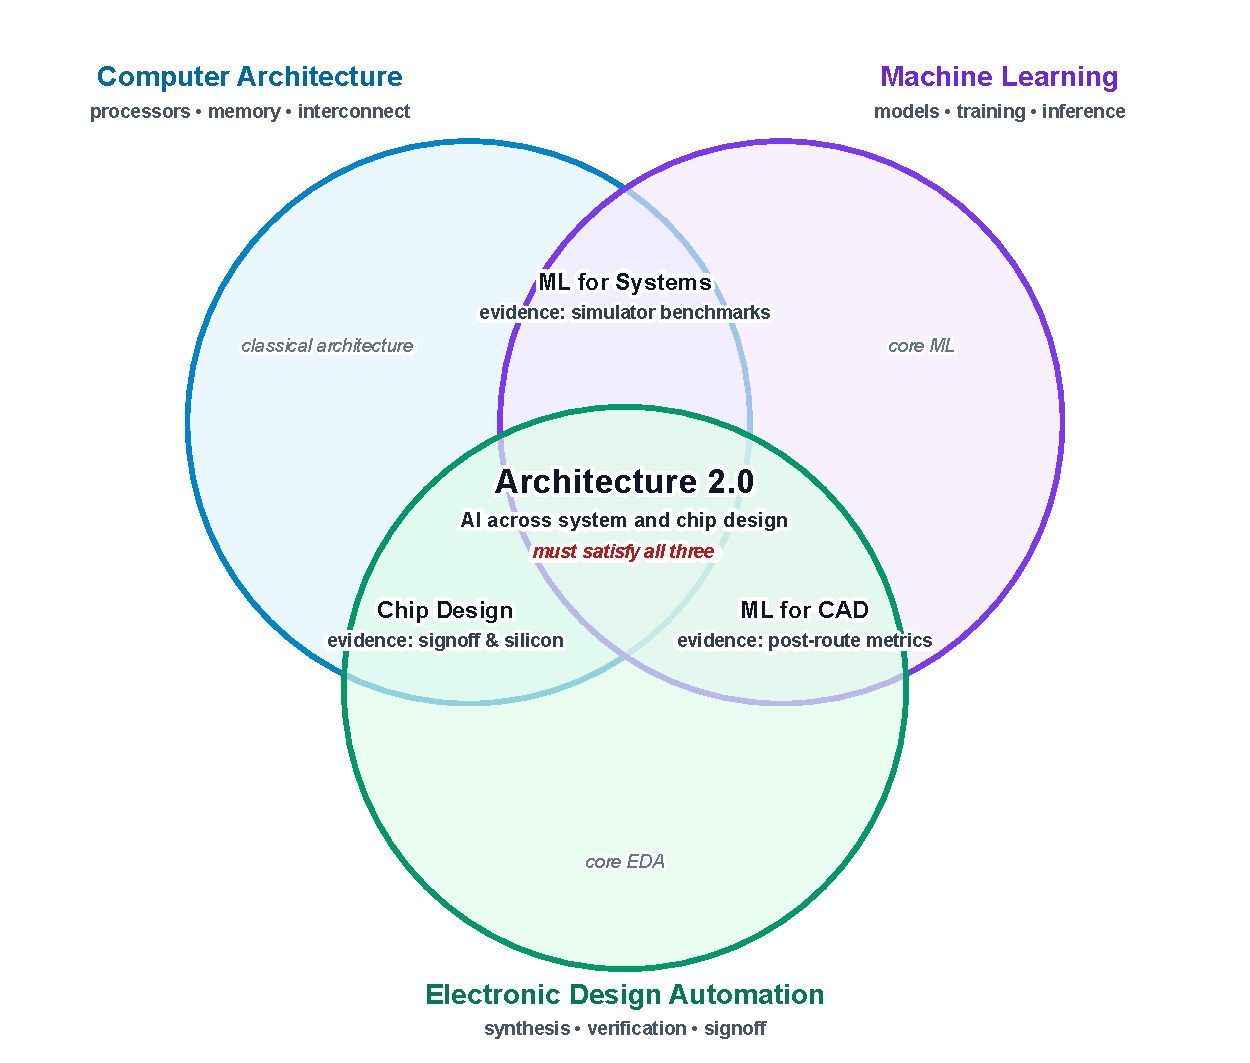
\includegraphics[width=\linewidth,height=4.65cm,keepaspectratio]{../book/images/fig-book-composition.pdf}
    \column{0.38\textwidth}
      \vspace{0.45cm}
      \begin{itemize}
        \item Architecture supplies the tradeoff and system boundary.
        \item ML supplies possible prediction, generation, and optimization methods.
        \item EDA supplies executable constraints and physical observations.
      \end{itemize}
  \end{columns}
\end{frame}

% 3
\begin{frame}{The one-sentence trap}
  \claim{A compact product request hides a full-stack architecture program.}
  \begin{columns}[T,onlytextwidth]
    \column{0.66\textwidth}
      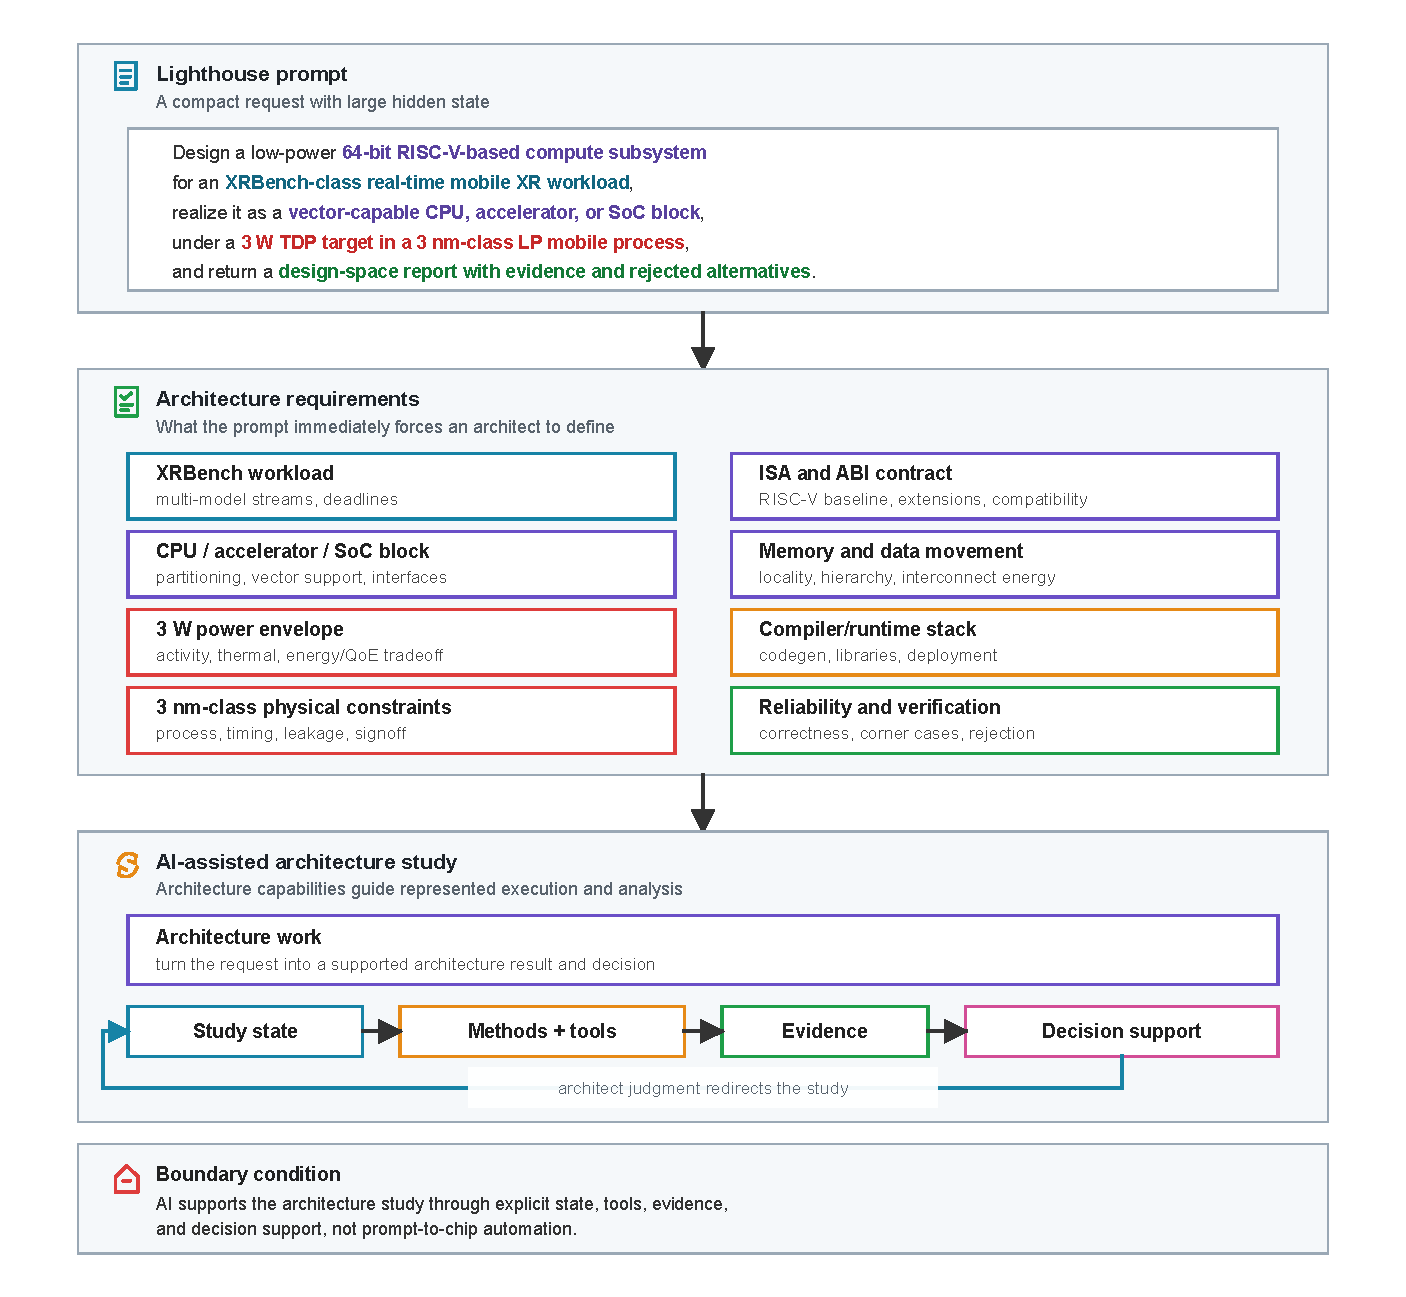
\includegraphics[width=\linewidth,height=4.55cm,keepaspectratio]{../book/chapters/01-moonshot/images/F1-moonshot-stack.pdf}
    \column{0.30\textwidth}
      \vspace{0.25cm}
      \tagbox{ArchGoldLight}{ArchGold}{Lighthouse target}
      \vspace{0.18cm}
      \begin{itemize}
        \item low-power, 64-bit RISC-V compute subsystem
        \item real-time mobile XR workloads
        \item software, RTL, physical, verification, and product constraints
      \end{itemize}
  \end{columns}
  \source{Architecture 2.0, Chapter 1; XRBench and ILLIXR ground the workload class.}
\end{frame}

% 4
\begin{frame}{Four different success claims}
  \claim{Output, architecture value, AI contribution, and moonshot completion are not interchangeable.}
  \begin{center}
  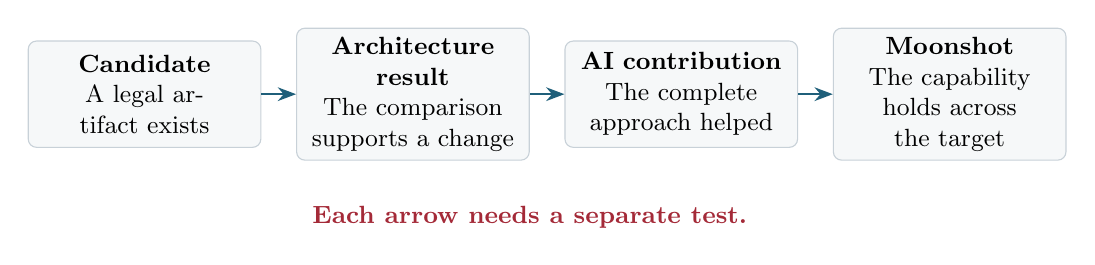
\begin{tikzpicture}[node distance=0.42cm and 0.44cm]
    \tikzset{claimstep/.style={rounded corners=3pt,draw=ArchLine,fill=ArchPanel,
      text width=2.72cm,minimum height=1.35cm,align=center,font=\small}}
    \node[claimstep] (a) {\textbf{Candidate}\\A legal artifact exists};
    \node[claimstep,right=of a] (b) {\textbf{Architecture result}\\The comparison supports a change};
    \node[claimstep,right=of b] (c) {\textbf{AI contribution}\\The complete approach helped};
    \node[claimstep,right=of c] (d) {\textbf{Moonshot}\\The capability holds across the target};
    \draw[-{Stealth},ArchBlue,thick] (a)--(b);
    \draw[-{Stealth},ArchBlue,thick] (b)--(c);
    \draw[-{Stealth},ArchBlue,thick] (c)--(d);
    \node[below=0.45cm of b.south east,align=center,text=ArchRed,font=\small\bfseries]
      {Each arrow needs a separate test.};
  \end{tikzpicture}
  \end{center}
\end{frame}

% 5
\begin{frame}{The Architecture 2.0 bet}
  \bigsep{Improve the architecture result, reduce the total cost of reaching a comparable result, or both.}
  \vspace{0.35cm}
  \begin{columns}[T,onlytextwidth]
    \column{0.31\textwidth}
      \tagbox{ArchBlueLight}{ArchBlue}{Architecture quality}
      \begin{itemize}
        \item performance, power, area
        \item reliability, security
        \item software and product fit
      \end{itemize}
    \column{0.31\textwidth}
      \tagbox{ArchGreenLight}{ArchGreen}{Total cost}
      \begin{itemize}
        \item model and tool calls
        \item queue and license time
        \item human setup, review, repair
      \end{itemize}
    \column{0.31\textwidth}
      \tagbox{ArchRedLight}{ArchRed}{Failure behavior}
      \begin{itemize}
        \item invalid candidates
        \item missed constraints
        \item unsafe or uncontrolled actions
      \end{itemize}
  \end{columns}
\end{frame}

% 6
\begin{frame}{Every efficiency lever adds obligations}
  \claim{Scaling gave way to specialization, composition, and cross-layer work.}
  \begin{center}
    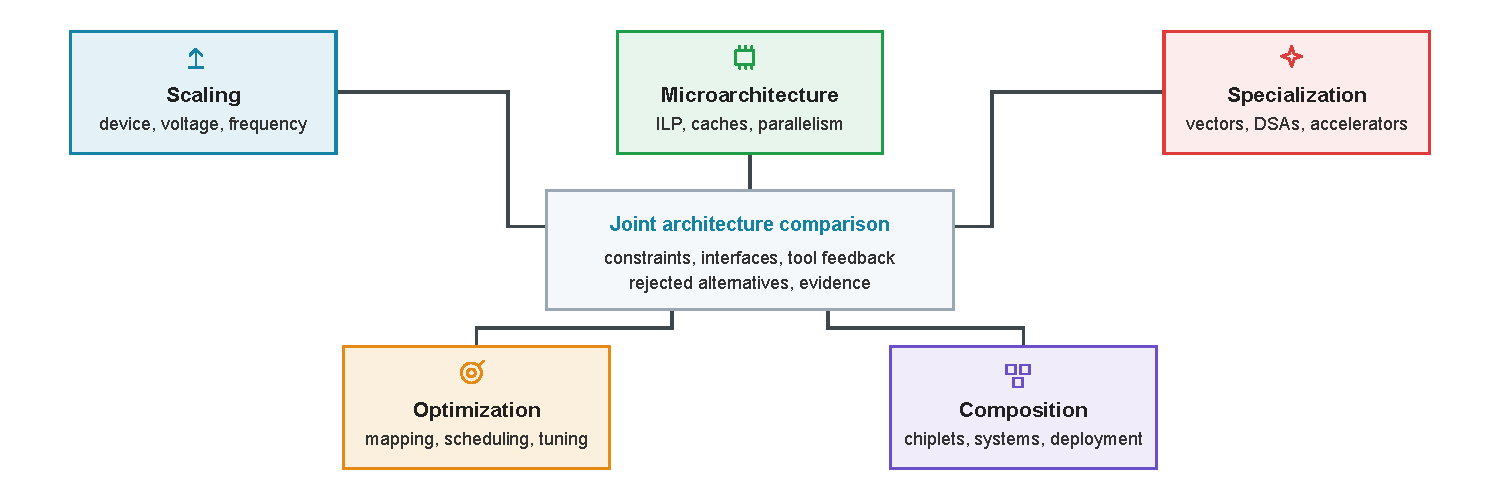
\includegraphics[width=0.84\linewidth,height=5.0cm,keepaspectratio]{../book/chapters/02-design-loop/images/F2-architecture-levers.pdf}
  \end{center}
  \source{Dennard scaling, Amdahl's law, dark silicon, chiplets, and warehouse-scale computing are established architecture results summarized in Chapter 2.}
\end{frame}

% 7
\begin{frame}{Data movement can dwarf arithmetic}
  \claim{The system boundary decides whether a local compute gain matters.}
  \begin{center}
  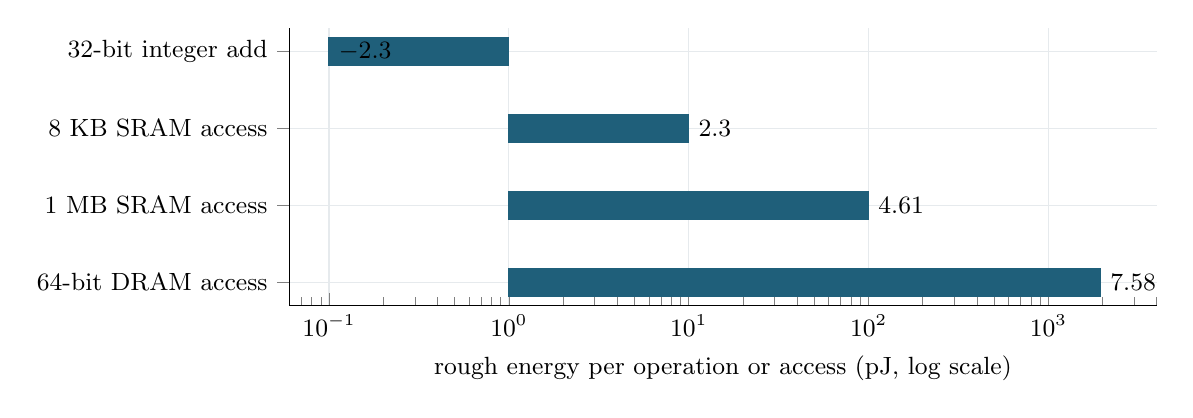
\begin{tikzpicture}
    \begin{axis}[
      width=12.6cm,height=5.1cm,
      xbar,xmode=log,
      xmin=0.06,xmax=4000,
      symbolic y coords={32-bit integer add,8 KB SRAM access,1 MB SRAM access,64-bit DRAM access},
      ytick=data,
      y dir=reverse,
      xlabel={rough energy per operation or access (pJ, log scale)},
      axis x line*=bottom,axis y line*=left,
      tick label style={font=\small},
      label style={font=\small},
      nodes near coords,
      nodes near coords align={horizontal},
      every node near coord/.append style={font=\small,anchor=west},
      bar width=10pt,
      grid=major,
      grid style={ArchLine!45},
    ]
      \addplot[fill=ArchBlue,draw=ArchBlue] coordinates
        {(0.1,32-bit integer add) (10,8 KB SRAM access) (100,1 MB SRAM access) (1950,64-bit DRAM access)};
    \end{axis}
  \end{tikzpicture}
  \end{center}
  \source{Horowitz, ISSCC 2014 rough 45 nm energy anchors. DRAM is plotted at the midpoint of the reported 1300--2600 pJ range; these are order-of-magnitude anchors, not current-node predictions.}
\end{frame}

% 8
\begin{frame}{Cost has moved beyond drawing the RTL}
  \claim{At advanced nodes, software, verification, and IP qualification can dominate estimated design cost.}
  \begin{columns}[T,onlytextwidth]
    \column{0.60\textwidth}
      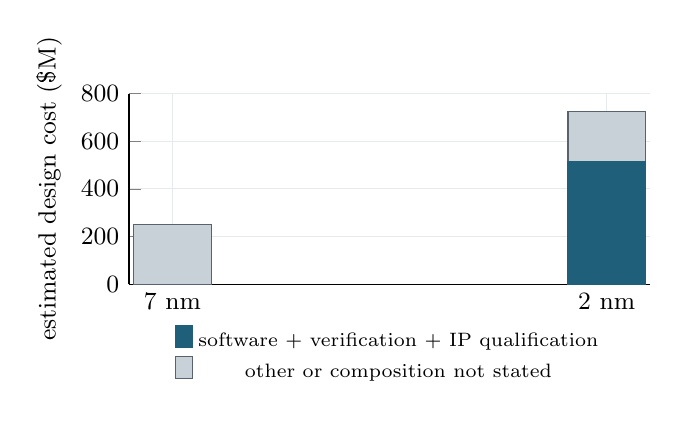
\begin{tikzpicture}
      \begin{axis}[
        width=8.2cm,height=4.0cm,
        ybar stacked,
        ymin=0,ymax=800,
        symbolic x coords={7 nm,2 nm},xtick=data,
        ylabel={estimated design cost (\$M)},
        bar width=28pt,
        tick label style={font=\small},
        label style={font=\small},
        legend style={font=\scriptsize,draw=none,at={(0.5,-0.18)},anchor=north,legend columns=1},
        axis x line*=bottom,axis y line*=left,
        grid=major,grid style={ArchLine!45},
      ]
        \addplot[fill=ArchBlue,draw=ArchBlue] coordinates {(7 nm,0) (2 nm,514.75)};
        \addplot[fill=ArchLine,draw=ArchMuted] coordinates {(7 nm,249) (2 nm,210.25)};
        \legend{software + verification + IP qualification,other or composition not stated}
      \end{axis}
      \end{tikzpicture}
    \column{0.35\textwidth}
      {\fontsize{34}{38}\selectfont\bfseries\color{ArchBlue}71\%\par}
      \vspace{0.1cm}
      \textbf{of the \$725M 2 nm estimate}\\
      was attributed to the combined software, verification, and IP-qualification categories.
      \vspace{0.4cm}

      \color{ArchMuted}\small The 7 nm composition was not published, so the chart does not invent it.
  \end{columns}
  \source{Arm Holdings, Form 424B4 (2023), reporting July 2022 IBS estimates: \$249M at 7 nm and \$725M at 2 nm.}
\end{frame}

% 9
\begin{frame}{Production can outpace examination}
  \claim{Faster candidate creation is useful only if evaluation and review can keep up.}
  \begin{center}
    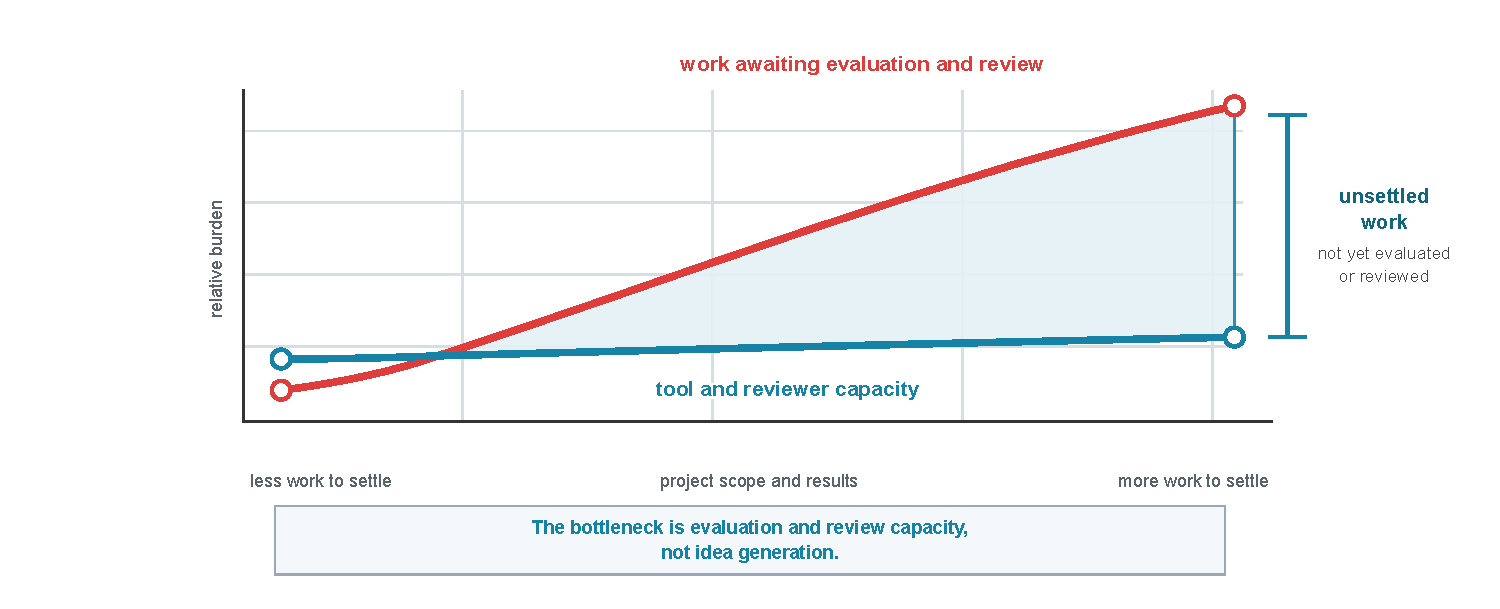
\includegraphics[width=0.88\linewidth,height=5.0cm,keepaspectratio]{../book/chapters/02-design-loop/images/F2-scissors-gap.pdf}
  \end{center}
\end{frame}

% 10
\begin{frame}{Diagnose the limiting work first}
  \claim{Different delays call for different interventions.}
  \begin{center}
  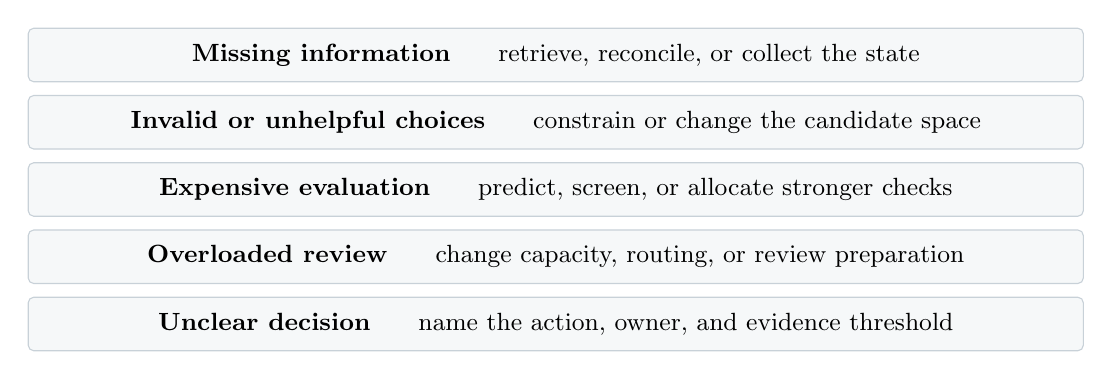
\begin{tikzpicture}[node distance=0.16cm]
    \tikzset{lane/.style={rounded corners=2pt,draw=ArchLine,minimum width=13.4cm,
      minimum height=0.68cm,align=left,font=\small,inner xsep=8pt}}
    \node[lane,fill=ArchPanel] (a) {\textbf{Missing information}\hspace{0.5cm} retrieve, reconcile, or collect the state};
    \node[lane,fill=ArchPanel,below=of a] (b) {\textbf{Invalid or unhelpful choices}\hspace{0.5cm} constrain or change the candidate space};
    \node[lane,fill=ArchPanel,below=of b] (c) {\textbf{Expensive evaluation}\hspace{0.5cm} predict, screen, or allocate stronger checks};
    \node[lane,fill=ArchPanel,below=of c] (d) {\textbf{Overloaded review}\hspace{0.5cm} change capacity, routing, or review preparation};
    \node[lane,fill=ArchPanel,below=of d] (e) {\textbf{Unclear decision}\hspace{0.5cm} name the action, owner, and evidence threshold};
  \end{tikzpicture}
  \end{center}
  \vspace{0.15cm}
  \begin{center}\color{ArchRed}\bfseries ``Use AI'' is not a diagnosis.\end{center}
\end{frame}

% 11
\begin{frame}{The object being engineered is the complete system}
  \begin{center}
    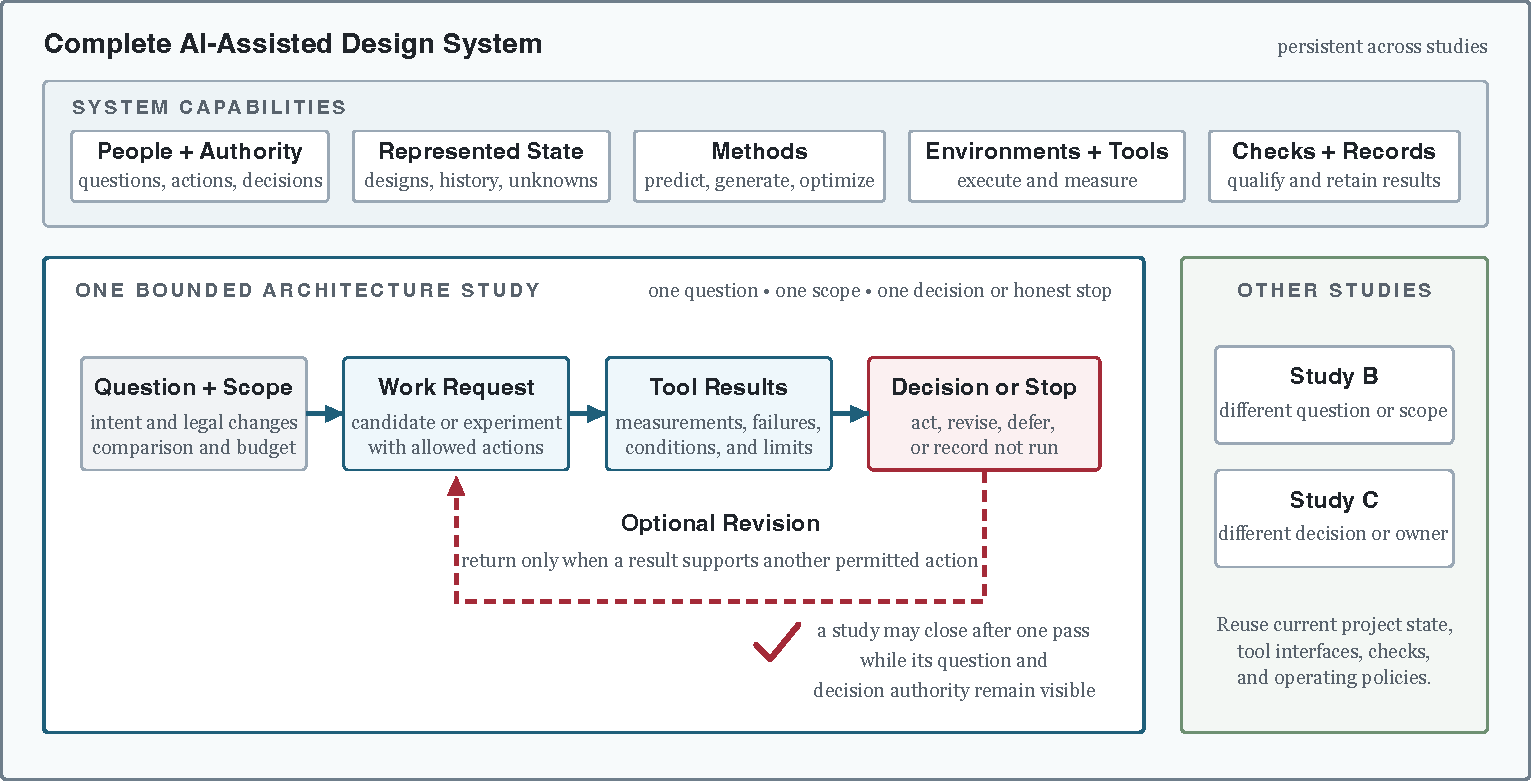
\includegraphics[width=0.93\linewidth,height=5.2cm,keepaspectratio]{../book/images/arch2-loop-diagram.pdf}
  \end{center}
\end{frame}

% 12
\begin{frame}{System, study, and loop are different}
  \claim{The loop is a possible behavior inside a study, not the whole thesis.}
  \begin{columns}[T,onlytextwidth]
    \column{0.31\textwidth}
      \tagbox{ArchBlueLight}{ArchBlue}{Complete system}
      \begin{itemize}
        \item persistent people, methods, tools, state, checks
        \item supports many studies
      \end{itemize}
    \column{0.31\textwidth}
      \tagbox{ArchGreenLight}{ArchGreen}{Bounded study}
      \begin{itemize}
        \item one question and scope
        \item one decision or honest stop
      \end{itemize}
    \column{0.31\textwidth}
      \tagbox{ArchGoldLight}{ArchGold}{Optional loop}
      \begin{itemize}
        \item another permitted action
        \item only when the result supports it
      \end{itemize}
  \end{columns}
\end{frame}

% 13
\begin{frame}{A bounded study connects question to decision}
  \begin{center}
    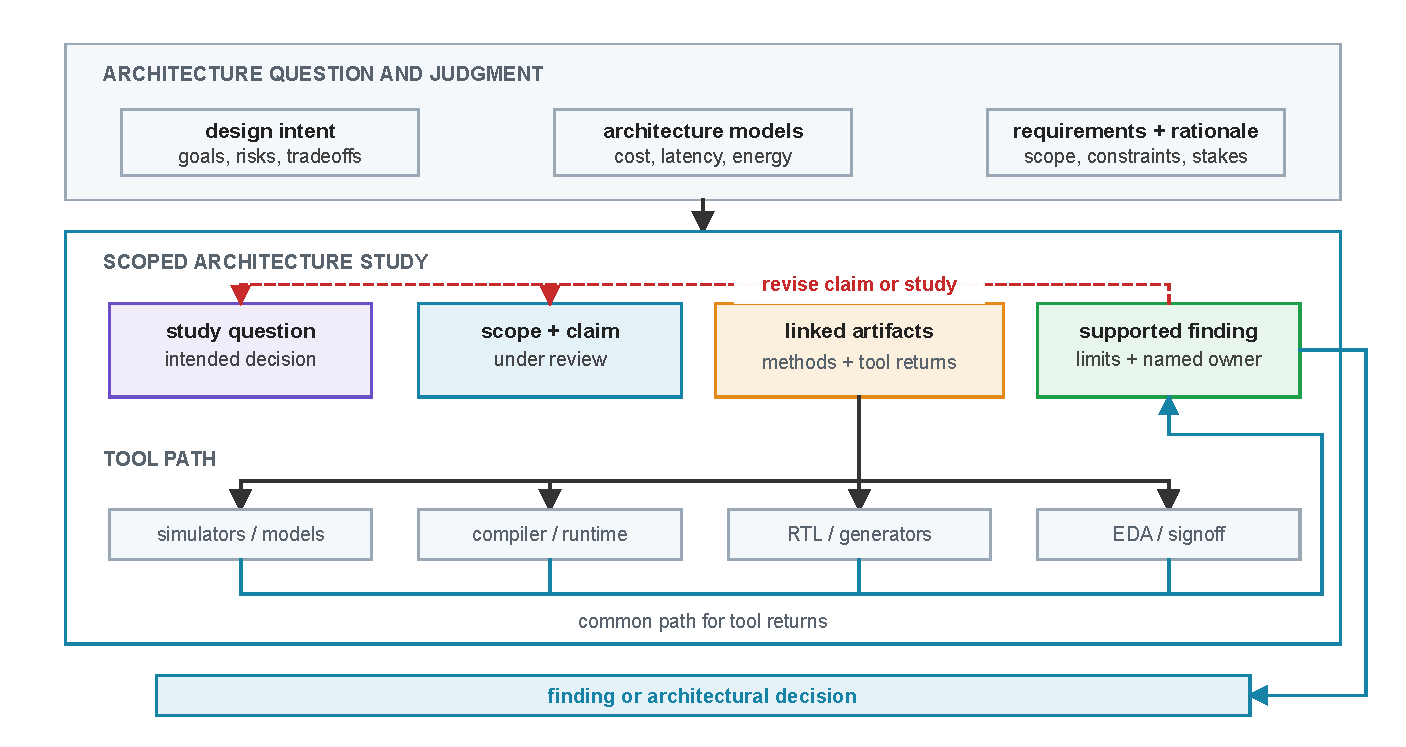
\includegraphics[width=0.88\linewidth,height=5.0cm,keepaspectratio]{../book/chapters/03-lifecycle/images/F4d-structured-layer-above-rtl.pdf}
  \end{center}
\end{frame}

% 14
\begin{frame}{Six distinct kinds of work}
  \claim{The stages are separated because they answer different questions and fail differently.}
  \begin{center}
    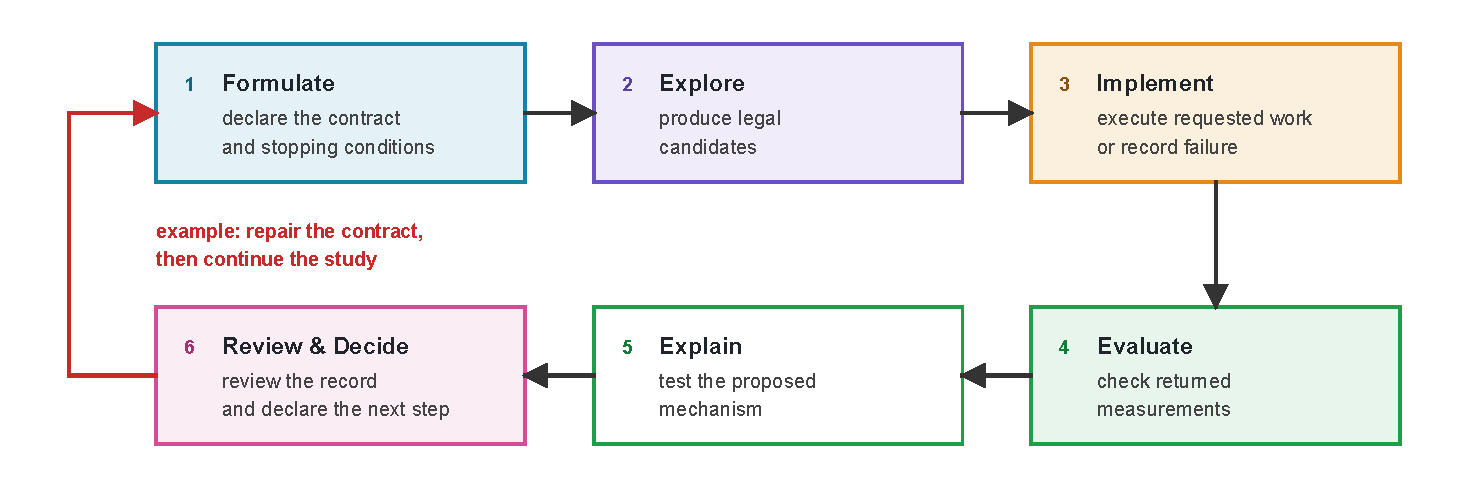
\includegraphics[width=0.94\linewidth,height=5.2cm,keepaspectratio]{../book/chapters/03-lifecycle/images/ch3-ontology-loop.pdf}
  \end{center}
\end{frame}

% 15
\begin{frame}{Repair the part that failed}
  \begin{center}
  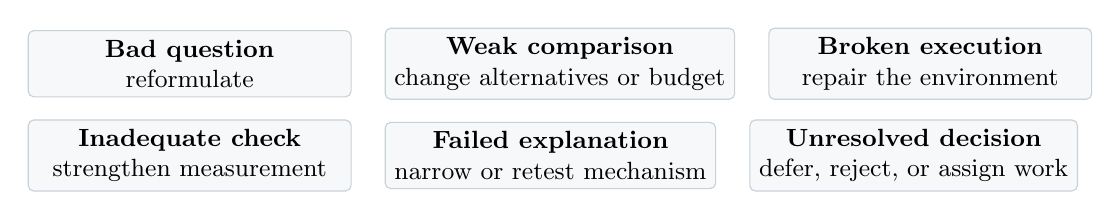
\begin{tikzpicture}[node distance=0.28cm and 0.42cm]
    \tikzset{r/.style={rounded corners=2pt,draw=ArchLine,fill=ArchPanel,
      minimum width=4.1cm,minimum height=0.82cm,align=center,font=\small}}
    \node[r] (a) {\textbf{Bad question}\\reformulate};
    \node[r,right=of a] (b) {\textbf{Weak comparison}\\change alternatives or budget};
    \node[r,right=of b] (c) {\textbf{Broken execution}\\repair the environment};
    \node[r,below=of a] (d) {\textbf{Inadequate check}\\strengthen measurement};
    \node[r,right=of d] (e) {\textbf{Failed explanation}\\narrow or retest mechanism};
    \node[r,right=of e] (f) {\textbf{Unresolved decision}\\defer, reject, or assign work};
  \end{tikzpicture}
  \end{center}
  \vspace{0.3cm}
  \begin{center}\color{ArchBlue}\bfseries Iteration should have a technical reason and a destination.\end{center}
\end{frame}

% 16
\begin{frame}{One record holds the comparison together}
  \claim{Another architect should be able to reconstruct what changed, what ran, what failed, and what the result supports.}
  \begin{center}
  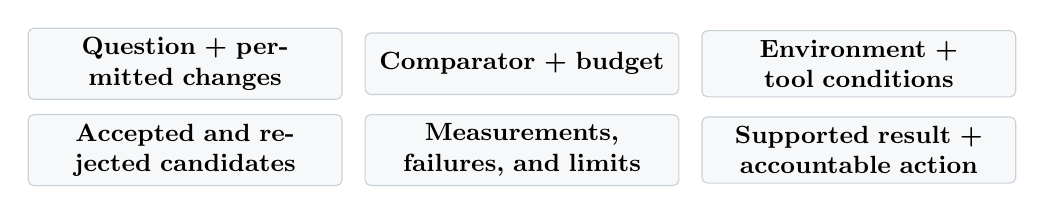
\begin{tikzpicture}[node distance=0.18cm and 0.28cm]
    \tikzset{record/.style={rounded corners=2pt,draw=ArchLine,fill=ArchPanel,
      text width=3.75cm,minimum height=0.78cm,align=center,font=\small}}
    \node[record] (a) {\textbf{Question + permitted changes}};
    \node[record,right=of a] (b) {\textbf{Comparator + budget}};
    \node[record,right=of b] (c) {\textbf{Environment + tool conditions}};
    \node[record,below=of a] (d) {\textbf{Accepted and rejected candidates}};
    \node[record,right=of d] (e) {\textbf{Measurements, failures, and limits}};
    \node[record,right=of e] (f) {\textbf{Supported result + accountable action}};
  \end{tikzpicture}
  \end{center}
  \vspace{0.25cm}
  \begin{center}\color{ArchBlue}\bfseries The record connects the technical argument; it is not the argument itself.\end{center}
\end{frame}

% 17
\begin{frame}{The project knows three different things}
  \begin{center}
  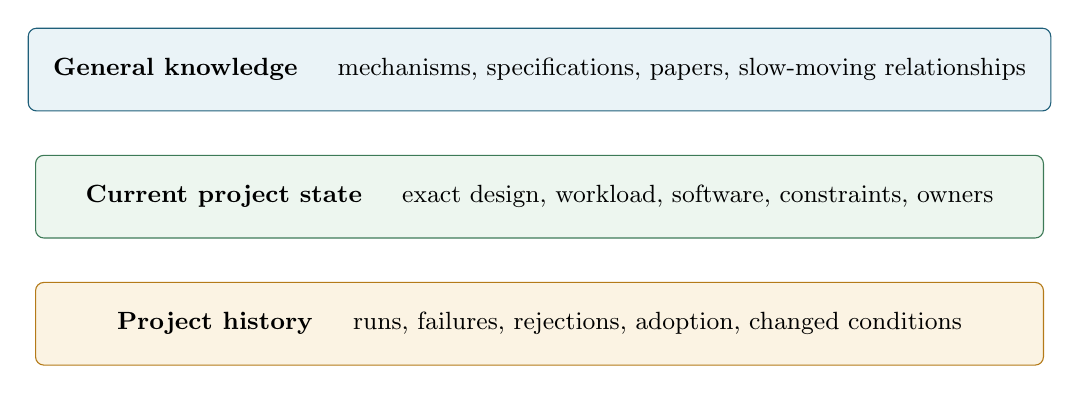
\begin{tikzpicture}[node distance=0.55cm]
    \tikzset{k/.style={rounded corners=3pt,minimum width=12.8cm,minimum height=1.05cm,
      align=left,inner xsep=9pt,font=\small}}
    \node[k,fill=ArchBlueLight,draw=ArchBlue] (a)
      {\textbf{General knowledge}\hspace{0.4cm} mechanisms, specifications, papers, slow-moving relationships};
    \node[k,fill=ArchGreenLight,draw=ArchGreen,below=of a] (b)
      {\textbf{Current project state}\hspace{0.4cm} exact design, workload, software, constraints, owners};
    \node[k,fill=ArchGoldLight,draw=ArchGold,below=of b] (c)
      {\textbf{Project history}\hspace{0.4cm} runs, failures, rejections, adoption, changed conditions};
  \end{tikzpicture}
  \end{center}
  \vspace{0.2cm}
  \begin{center}\color{ArchRed}\bfseries A model's general knowledge is not live project state.\end{center}
\end{frame}

% 18
\begin{frame}{Observation sources are not interchangeable}
  \claim{Choose the source by the property the study must observe, not by a single fidelity ranking.}
  \begin{center}
    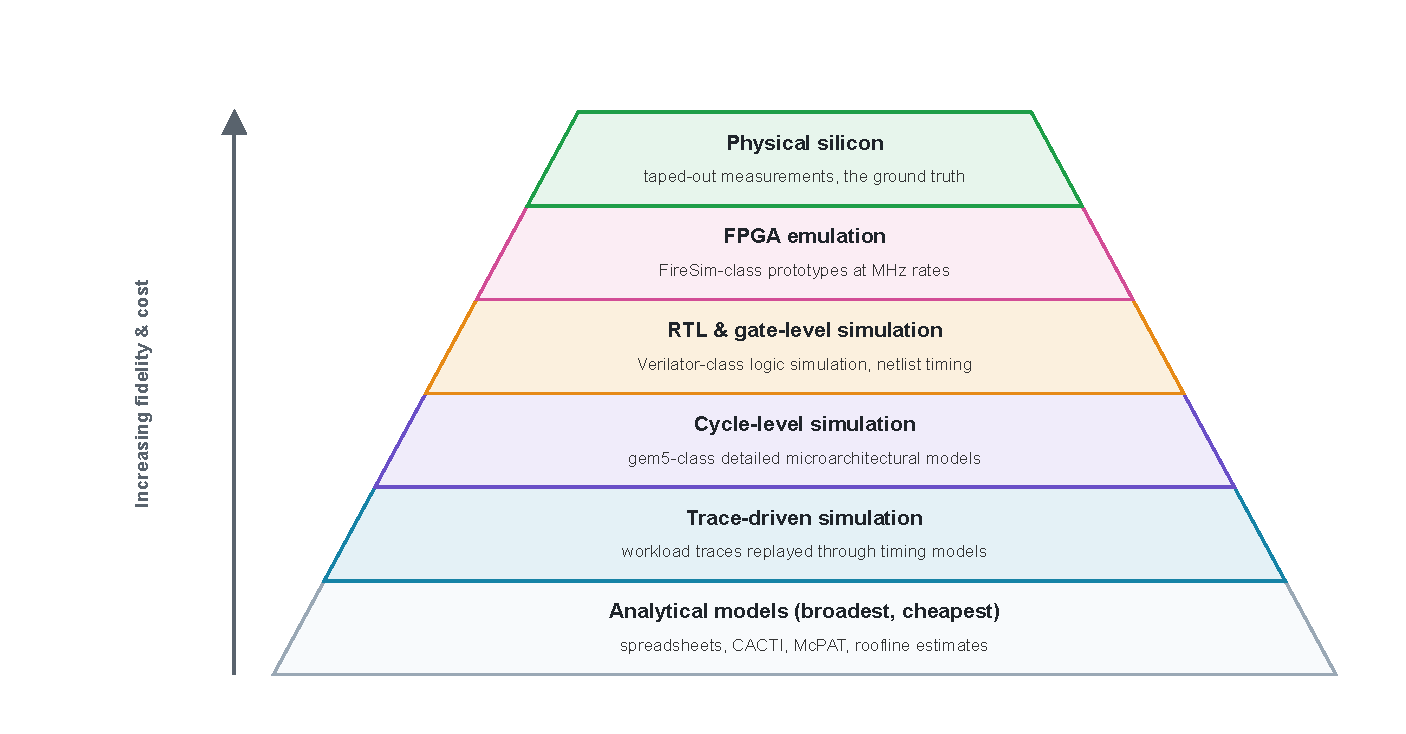
\includegraphics[width=0.88\linewidth,height=5.0cm,keepaspectratio]{../book/chapters/04-representations/images/F4-data-pyramid.pdf}
  \end{center}
\end{frame}

% 19
\begin{frame}{An architecture sample can be expensive}
  \claim{Data acquisition is part of the architecture method, not background plumbing.}
  \begin{center}
  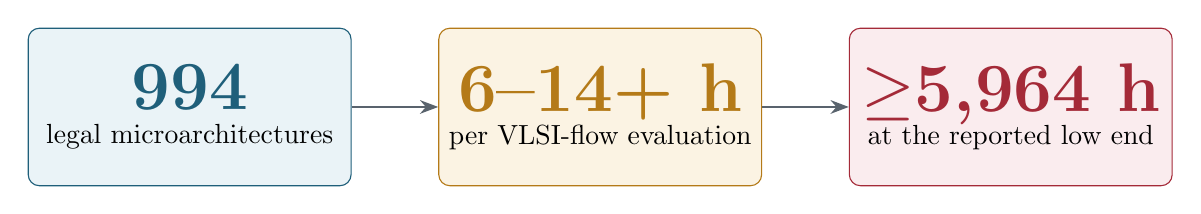
\begin{tikzpicture}
    \node[rounded corners=4pt,fill=ArchBlueLight,draw=ArchBlue,
      minimum width=4.1cm,minimum height=2.0cm,align=center] (a)
      {{\fontsize{30}{34}\selectfont\bfseries\color{ArchBlue}994}\\legal microarchitectures};
    \node[rounded corners=4pt,fill=ArchGoldLight,draw=ArchGold,
      minimum width=4.1cm,minimum height=2.0cm,align=center,right=1.1cm of a] (b)
      {{\fontsize{30}{34}\selectfont\bfseries\color{ArchGold}6--14+ h}\\per VLSI-flow evaluation};
    \node[rounded corners=4pt,fill=ArchRedLight,draw=ArchRed,
      minimum width=4.1cm,minimum height=2.0cm,align=center,right=1.1cm of b] (c)
      {{\fontsize{25}{29}\selectfont\bfseries\color{ArchRed}$\geq$5,964 h}\\at the reported low end};
    \draw[-{Stealth},ArchMuted,thick] (a)--(b);
    \draw[-{Stealth},ArchMuted,thick] (b)--(c);
  \end{tikzpicture}
  \end{center}
  \vspace{0.3cm}
  \begin{center}\small Ten analytical calls, ten cycle simulations, and ten physical-design runs are not ten equivalent samples.\end{center}
  \source{BOOM-Explorer: Bai et al., ISCA 2021. The final value is a lower-bound multiplication of the reported sample count and low-end runtime.}
\end{frame}

% 20
\begin{frame}{Representation determines reachable designs}
  \claim{A legal proposal can still be invalid when project state and tool-facing artifacts disagree.}
  \begin{center}
    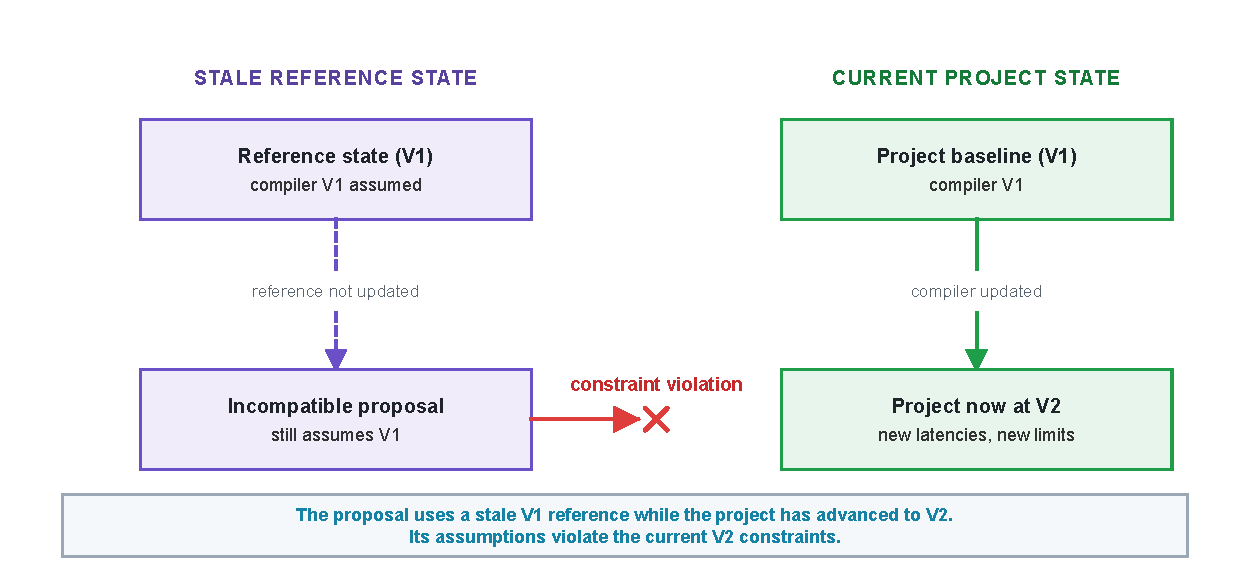
\includegraphics[width=0.87\linewidth,height=4.75cm,keepaspectratio]{../book/chapters/04-representations/images/F4b-split-brain-causality.pdf}
  \end{center}
\end{frame}

% 21
\begin{frame}{Role comes before method}
  \claim{Do not collapse an engineering job, a method family, and an implementation into ``the AI.''}
  \begin{center}
  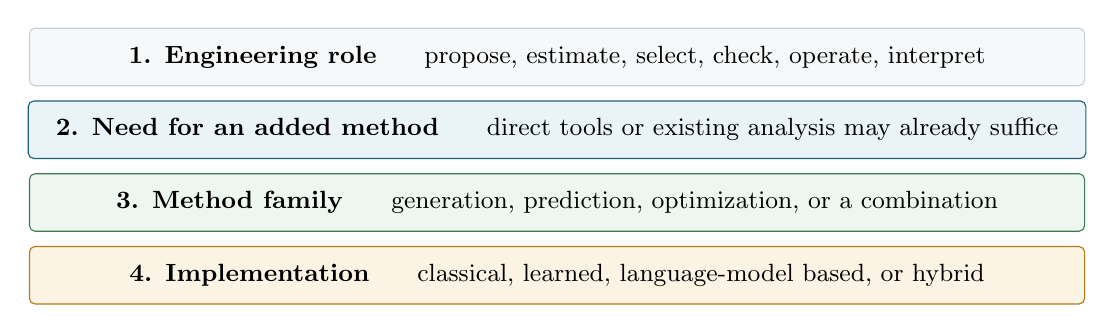
\begin{tikzpicture}[node distance=0.18cm]
    \tikzset{s/.style={rounded corners=2pt,minimum width=13.4cm,minimum height=0.73cm,
      align=left,inner xsep=10pt,font=\small}}
    \node[s,fill=ArchPanel,draw=ArchLine] (a) {\textbf{1. Engineering role}\hspace{0.5cm} propose, estimate, select, check, operate, interpret};
    \node[s,fill=ArchBlueLight,draw=ArchBlue,below=of a] (b) {\textbf{2. Need for an added method}\hspace{0.5cm} direct tools or existing analysis may already suffice};
    \node[s,fill=ArchGreenLight,draw=ArchGreen,below=of b] (c) {\textbf{3. Method family}\hspace{0.5cm} generation, prediction, optimization, or a combination};
    \node[s,fill=ArchGoldLight,draw=ArchGold,below=of c] (d) {\textbf{4. Implementation}\hspace{0.5cm} classical, learned, language-model based, or hybrid};
  \end{tikzpicture}
  \end{center}
\end{frame}

% 22
\begin{frame}{Use the smallest sufficient approach}
  \begin{center}
  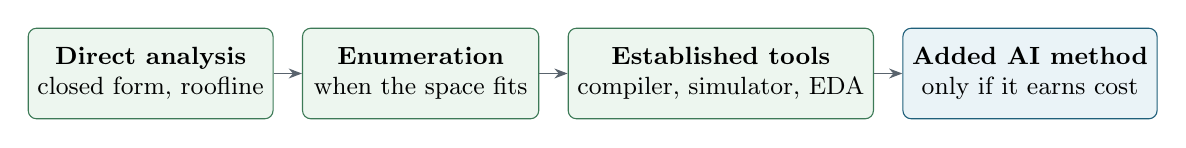
\begin{tikzpicture}[node distance=0.36cm]
    \tikzset{m/.style={rounded corners=3pt,draw=ArchLine,minimum width=3.0cm,
      minimum height=1.15cm,align=center,font=\small}}
    \node[m,fill=ArchGreenLight,draw=ArchGreen] (a) {\textbf{Direct analysis}\\closed form, roofline};
    \node[m,fill=ArchGreenLight,draw=ArchGreen,right=of a] (b) {\textbf{Enumeration}\\when the space fits};
    \node[m,fill=ArchGreenLight,draw=ArchGreen,right=of b] (c) {\textbf{Established tools}\\compiler, simulator, EDA};
    \node[m,fill=ArchBlueLight,draw=ArchBlue,right=of c] (d) {\textbf{Added AI method}\\only if it earns cost};
    \draw[-{Stealth},ArchMuted] (a)--(b);
    \draw[-{Stealth},ArchMuted] (b)--(c);
    \draw[-{Stealth},ArchMuted] (c)--(d);
  \end{tikzpicture}
  \end{center}
  \vspace{0.55cm}
  \bigsep{``No added AI'' is a valid architecture-method decision.}
\end{frame}

% 23
\begin{frame}{Three method families}
  \claim{Start from what is missing, not from a fixed prediction--generation--optimization sequence.}
  \begin{center}
  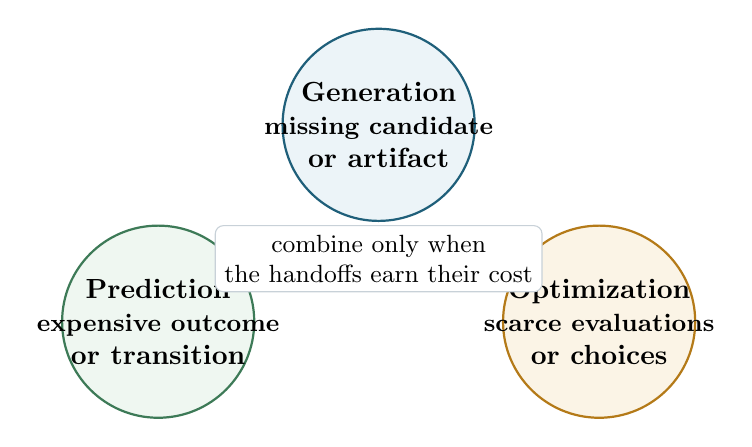
\begin{tikzpicture}
    \coordinate (g) at (0,1.55);
    \coordinate (p) at (-2.8,-0.95);
    \coordinate (o) at (2.8,-0.95);
    \fill[ArchBlueLight,opacity=.9] (g) circle (1.22cm);
    \fill[ArchGreenLight,opacity=.9] (p) circle (1.22cm);
    \fill[ArchGoldLight,opacity=.9] (o) circle (1.22cm);
    \draw[ArchBlue,thick] (g) circle (1.22cm);
    \draw[ArchGreen,thick] (p) circle (1.22cm);
    \draw[ArchGold,thick] (o) circle (1.22cm);
    \node[align=center,font=\bfseries] at (g) {Generation\\\small missing candidate\\or artifact};
    \node[align=center,font=\bfseries] at (p) {Prediction\\\small expensive outcome\\or transition};
    \node[align=center,font=\bfseries] at (o) {Optimization\\\small scarce evaluations\\or choices};
    \node[rounded corners=3pt,fill=white,draw=ArchLine,align=center,font=\small] at (0,-0.15)
      {combine only when\\the handoffs earn their cost};
  \end{tikzpicture}
  \end{center}
\end{frame}

% 24
\begin{frame}{Generation expands the candidate set}
  \claim{Attempted, executable, correct, and useful are different conditions.}
  \begin{center}
  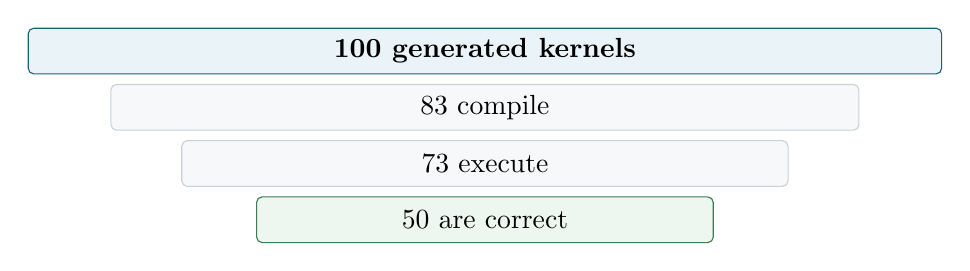
\begin{tikzpicture}[node distance=0.12cm]
    \node[rounded corners=2pt,
      minimum width=11.6cm,minimum height=0.58cm,fill=ArchBlueLight,draw=ArchBlue] (a)
      {\textbf{100 generated kernels}};
    \node[rounded corners=2pt,
      minimum width=9.5cm,minimum height=0.58cm,fill=ArchPanel,draw=ArchLine,below=of a] (b)
      {83 compile};
    \node[rounded corners=2pt,
      minimum width=7.7cm,minimum height=0.58cm,fill=ArchPanel,draw=ArchLine,below=of b] (c)
      {73 execute};
    \node[rounded corners=2pt,
      minimum width=5.8cm,minimum height=0.58cm,fill=ArchGreenLight,draw=ArchGreen,below=of c] (d)
      {50 are correct};
  \end{tikzpicture}
  \end{center}
  \vspace{0.16cm}
  \begin{center}\color{ArchRed}\bfseries Correct and faster than the baseline is narrower again.\end{center}
  \source{KernelBench, Ouyang et al. (2025), separate 100-kernel error-analysis sample. Per-model one-shot results in the paper show the same attempted $\rightarrow$ correct $\rightarrow$ correct-and-faster narrowing.}
\end{frame}

% 25
\begin{frame}{Prediction trades cost for a support assumption}
  \claim{A cheap predictor helps only where its error is acceptable for the decision it screens.}
  \begin{center}
  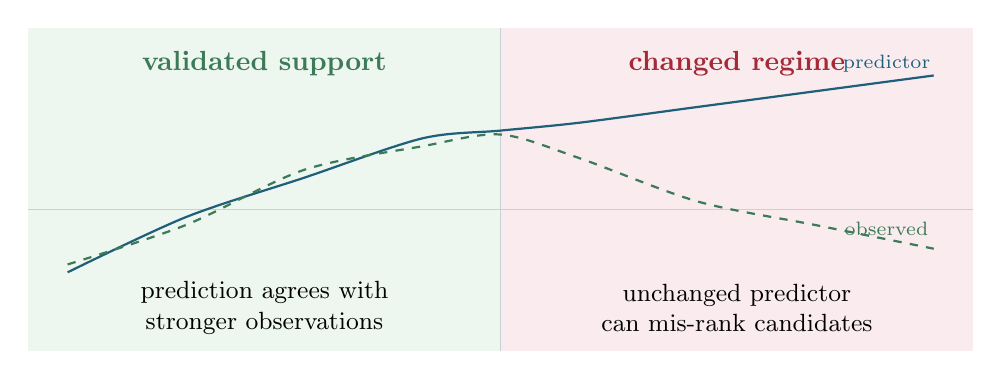
\begin{tikzpicture}
    \fill[ArchGreenLight] (-6,-1.8) rectangle (0,2.3);
    \fill[ArchRedLight] (0,-1.8) rectangle (6,2.3);
    \draw[ArchLine] (-6,0) -- (6,0);
    \draw[ArchLine] (0,-1.8) -- (0,2.3);
    \draw[ArchBlue,thick] plot[smooth] coordinates {(-5.5,-.8) (-4,-.1) (-2.5,.4) (-1,.9) (0,1.0) (1,1.1) (2.5,1.3) (4,1.5) (5.5,1.7)};
    \draw[ArchGreen,thick,dashed] plot[smooth] coordinates {(-5.5,-.7) (-4,-.2) (-2.5,.5) (-1,.8) (0,.95) (1,.65) (2.5,.1) (4,-.2) (5.5,-.5)};
    \node[font=\bfseries,text=ArchGreen] at (-3,1.85) {validated support};
    \node[font=\bfseries,text=ArchRed] at (3,1.85) {changed regime};
    \node[font=\small,align=center] at (-3,-1.25) {prediction agrees with\\stronger observations};
    \node[font=\small,align=center] at (3,-1.25) {unchanged predictor\\can mis-rank candidates};
    \node[font=\scriptsize,text=ArchBlue] at (4.9,1.85) {predictor};
    \node[font=\scriptsize,text=ArchGreen] at (4.9,-.25) {observed};
  \end{tikzpicture}
  \end{center}
  \source{Constructed teaching illustration; Chapter 5 develops calibration and support limits.}
\end{frame}

% 26
\begin{frame}{A world model is a scoped predictor}
  \claim{It predicts consequences of state and action; it is not a fourth method family or authoritative project state.}
  \begin{center}
    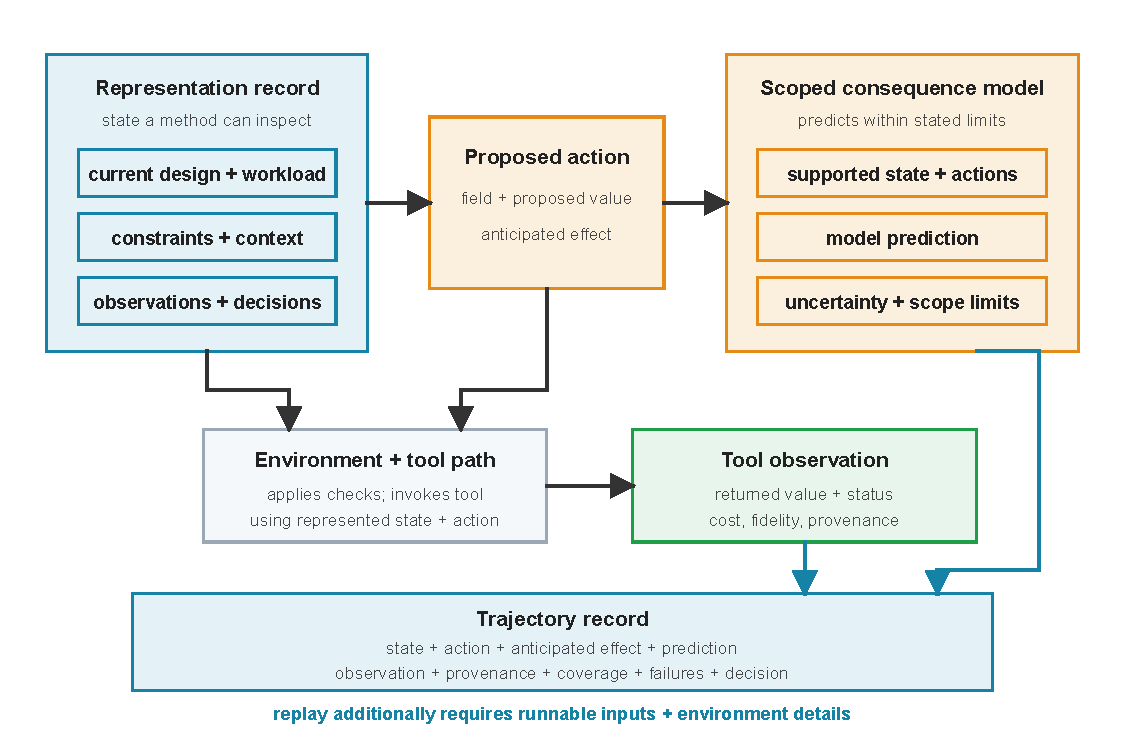
\includegraphics[width=0.86\linewidth,height=4.75cm,keepaspectratio]{../book/chapters/05-methods/images/F5-architecture-world-model.pdf}
  \end{center}
\end{frame}

% 27
\begin{frame}{Optimization allocates scarce evaluations}
  \claim{When feedback is expensive, the next evaluation matters more than another unmeasured candidate.}
  \begin{center}
  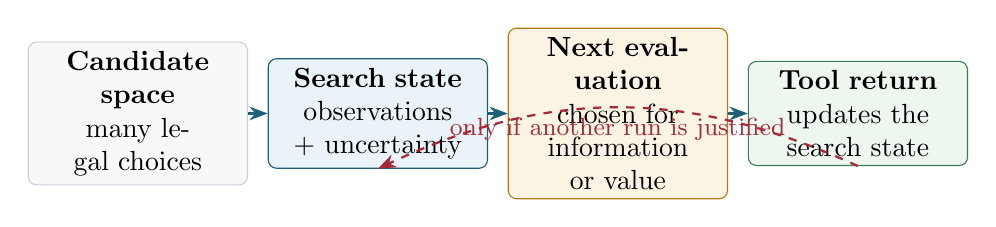
\begin{tikzpicture}[node distance=0.25cm]
    \node[rounded corners=3pt,fill=ArchPanel,draw=ArchLine,text width=2.55cm,minimum height=1.2cm,align=center] (a)
      {\textbf{Candidate space}\\many legal choices};
    \node[rounded corners=3pt,fill=ArchBlueLight,draw=ArchBlue,text width=2.55cm,minimum height=1.2cm,align=center,right=of a] (b)
      {\textbf{Search state}\\observations + uncertainty};
    \node[rounded corners=3pt,fill=ArchGoldLight,draw=ArchGold,text width=2.55cm,minimum height=1.2cm,align=center,right=of b] (c)
      {\textbf{Next evaluation}\\chosen for information or value};
    \node[rounded corners=3pt,fill=ArchGreenLight,draw=ArchGreen,text width=2.55cm,minimum height=1.2cm,align=center,right=of c] (d)
      {\textbf{Tool return}\\updates the search state};
    \draw[-{Stealth},ArchBlue,thick] (a)--(b);
    \draw[-{Stealth},ArchBlue,thick] (b)--(c);
    \draw[-{Stealth},ArchBlue,thick] (c)--(d);
    \draw[-{Stealth},ArchRed,thick,dashed] (d.south) to[bend right=25] node[below,font=\small,text=ArchRed]{only if another run is justified} (b.south);
  \end{tikzpicture}
  \end{center}
\end{frame}

% 28
\begin{frame}{Method handoffs must earn their cost}
  \begin{center}
  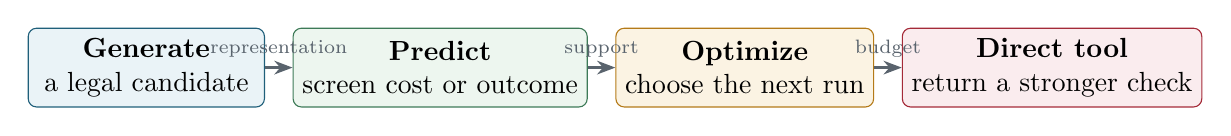
\begin{tikzpicture}[node distance=0.35cm]
    \tikzset{c/.style={rounded corners=3pt,draw=ArchLine,minimum width=3.0cm,minimum height=1.0cm,align=center}}
    \node[c,fill=ArchBlueLight,draw=ArchBlue] (g) {\textbf{Generate}\\a legal candidate};
    \node[c,fill=ArchGreenLight,draw=ArchGreen,right=of g] (p) {\textbf{Predict}\\screen cost or outcome};
    \node[c,fill=ArchGoldLight,draw=ArchGold,right=of p] (o) {\textbf{Optimize}\\choose the next run};
    \node[c,fill=ArchRedLight,draw=ArchRed,right=of o] (t) {\textbf{Direct tool}\\return a stronger check};
    \draw[-{Stealth},ArchMuted,thick] (g)-- node[above,font=\scriptsize]{representation} (p);
    \draw[-{Stealth},ArchMuted,thick] (p)-- node[above,font=\scriptsize]{support} (o);
    \draw[-{Stealth},ArchMuted,thick] (o)-- node[above,font=\scriptsize]{budget} (t);
  \end{tikzpicture}
  \end{center}
  \vspace{0.45cm}
  \begin{columns}[T,onlytextwidth]
    \column{0.48\textwidth}
      \tagbox{ArchGreenLight}{ArchGreen}{Justified}
      \begin{itemize}
        \item each stage removes more cost than it adds
        \item rejected candidates and failures stay visible
      \end{itemize}
    \column{0.48\textwidth}
      \tagbox{ArchRedLight}{ArchRed}{Not justified}
      \begin{itemize}
        \item more components without a named bottleneck
        \item a cheap proxy replaces the decisive check
      \end{itemize}
  \end{columns}
\end{frame}

% 29
\begin{frame}{An environment is more than a simulator}
  \begin{center}
    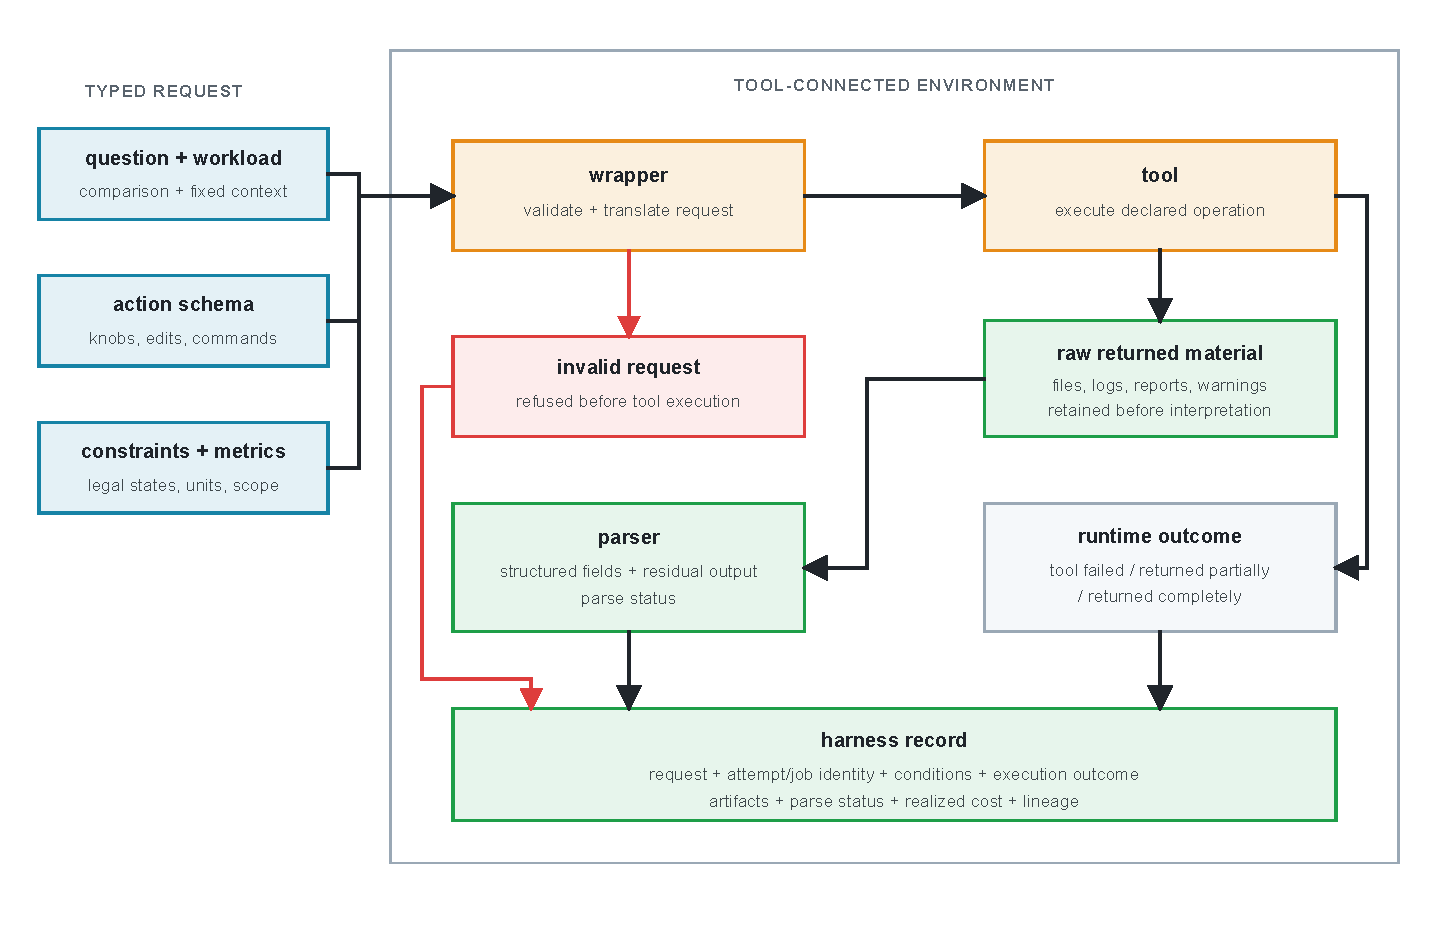
\includegraphics[width=0.91\linewidth,height=5.05cm,keepaspectratio]{../book/chapters/06-environments/images/F6-environment-tool-interface.pdf}
  \end{center}
\end{frame}

% 30
\begin{frame}{Identity must survive every tool}
  \claim{A successful command is not enough to reconstruct a result.}
  \begin{center}
    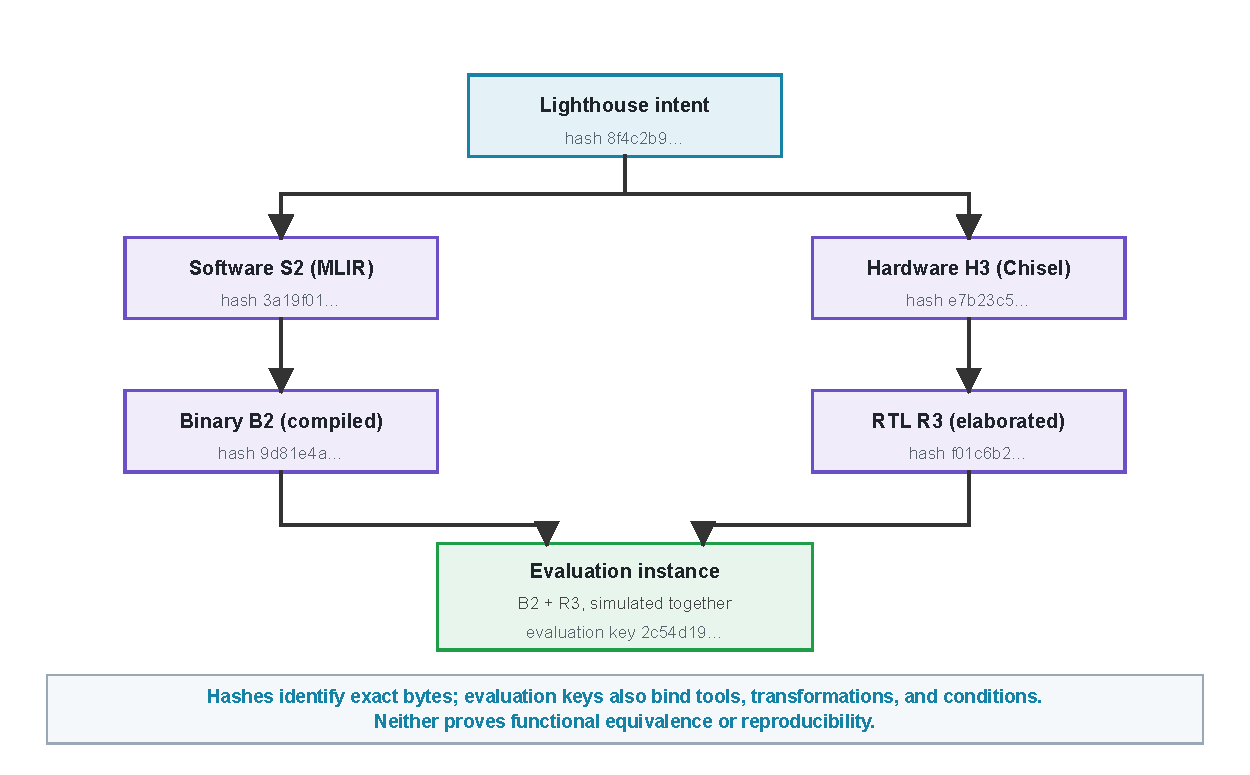
\includegraphics[width=0.90\linewidth,height=4.9cm,keepaspectratio]{../book/chapters/06-environments/images/F5-artifact-lineage.pdf}
  \end{center}
\end{frame}

% 31
\begin{frame}{A return is not yet a measurement}
  \claim{Qualification, comparison, and interpretation give a tool return its meaning.}
  \begin{center}
  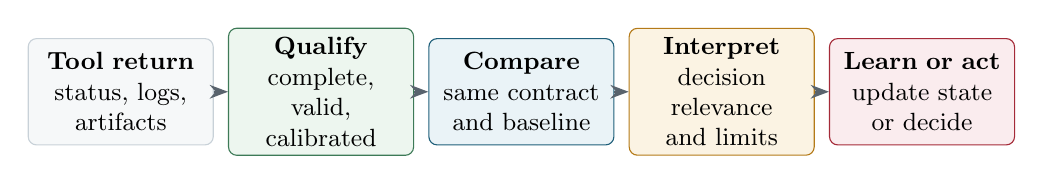
\begin{tikzpicture}[node distance=0.18cm]
    \tikzset{measurestage/.style={rounded corners=3pt,minimum width=2.35cm,text width=2.05cm,
      minimum height=1.35cm,align=center,inner xsep=3pt,font=\small}}
    \node[measurestage,fill=ArchPanel,draw=ArchLine] (a) {\textbf{Tool return}\\status, logs,\\artifacts};
    \node[measurestage,fill=ArchGreenLight,draw=ArchGreen,right=of a] (b) {\textbf{Qualify}\\complete, valid,\\calibrated};
    \node[measurestage,fill=ArchBlueLight,draw=ArchBlue,right=of b] (c) {\textbf{Compare}\\same contract\\and baseline};
    \node[measurestage,fill=ArchGoldLight,draw=ArchGold,right=of c] (d) {\textbf{Interpret}\\decision relevance\\and limits};
    \node[measurestage,fill=ArchRedLight,draw=ArchRed,right=of d] (e) {\textbf{Learn or act}\\update state\\or decide};
    \draw[-{Stealth},ArchMuted,thick] (a)--(b);
    \draw[-{Stealth},ArchMuted,thick] (b)--(c);
    \draw[-{Stealth},ArchMuted,thick] (c)--(d);
    \draw[-{Stealth},ArchMuted,thick] (d)--(e);
  \end{tikzpicture}
  \end{center}
  \vspace{0.48cm}
  \bigsep{If qualification fails, return to the tool or environment. Do not report a measurement.}
\end{frame}

% 32
\begin{frame}{Formal and simulation answer different questions}
  \begin{columns}[T,onlytextwidth]
    \column{0.47\textwidth}
      \tagbox{ArchBlueLight}{ArchBlue}{Formal}
      \begin{itemize}
        \item proves or falsifies a stated property
        \item under a model and assumptions
        \item may be inconclusive or time out
      \end{itemize}
    \column{0.47\textwidth}
      \tagbox{ArchGreenLight}{ArchGreen}{Simulation}
      \begin{itemize}
        \item observes exercised behavior
        \item under selected stimuli and configuration
        \item cannot exhaust a modern design
      \end{itemize}
  \end{columns}
  \vspace{0.38cm}
  \bigsep{Neither check repairs an incomplete requirement or system boundary.}
\end{frame}

% 33
\begin{frame}{Another model is not an independent check}
  \claim{Independence comes from a materially different observation path, not another fluent answer.}
  \begin{center}
    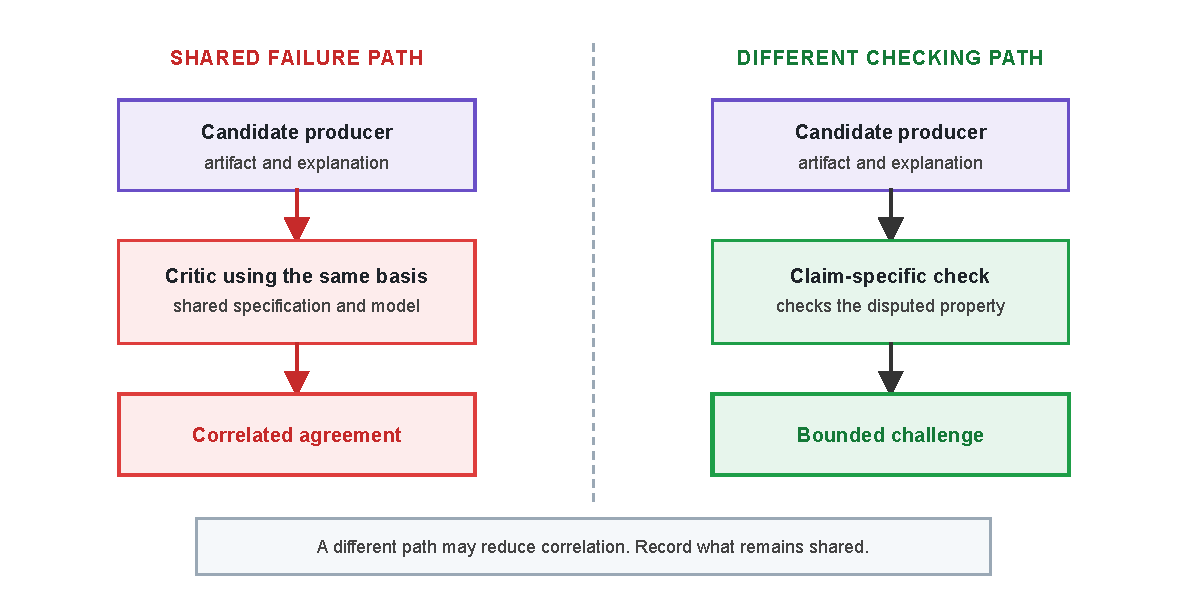
\includegraphics[width=0.87\linewidth,height=4.7cm,keepaspectratio]{../book/chapters/07-feedback/images/ch7_independent_checks.pdf}
  \end{center}
\end{frame}

% 34
\begin{frame}{One complete study must resolve four judgments}
  \claim{Architecture outcome, AI contribution, mechanism, and action remain separate.}
  \begin{center}
    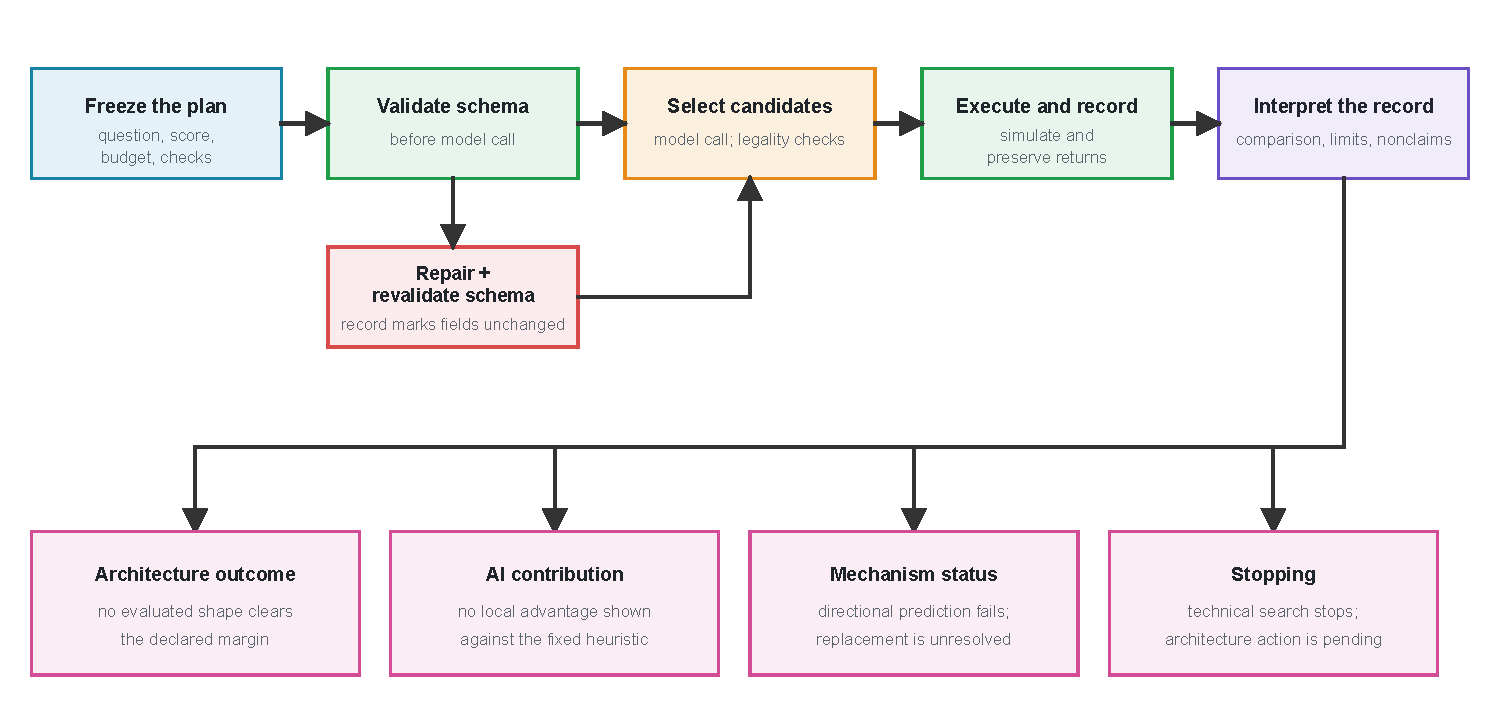
\includegraphics[width=0.91\linewidth,height=4.85cm,keepaspectratio]{../book/chapters/08-running-the-loop/images/ch8_design_loop_workflow.pdf}
  \end{center}
\end{frame}

% 35
\begin{frame}{Equal simulator budgets produced a tie}
  \claim{Neither proposal arm found a nonbaseline shape that cleared the predeclared 1\% margin.}
  \begin{center}
  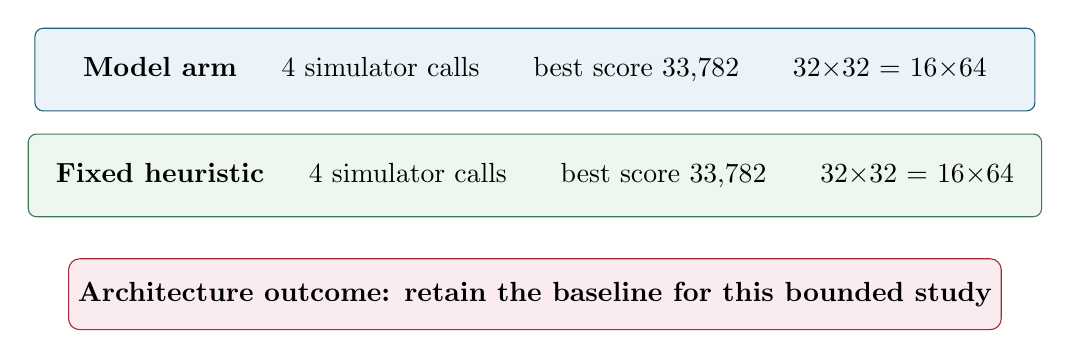
\begin{tikzpicture}[node distance=0.28cm]
    \tikzset{row/.style={rounded corners=3pt,minimum width=12.7cm,minimum height=1.05cm,align=left,inner xsep=10pt}}
    \node[row,fill=ArchBlueLight,draw=ArchBlue] (a)
      {\textbf{Model arm}\hspace{0.45cm} 4 simulator calls \hspace{0.45cm} best score 33,782 \hspace{0.45cm} 32$\times$32 = 16$\times$64};
    \node[row,fill=ArchGreenLight,draw=ArchGreen,below=of a] (b)
      {\textbf{Fixed heuristic}\hspace{0.45cm} 4 simulator calls \hspace{0.45cm} best score 33,782 \hspace{0.45cm} 32$\times$32 = 16$\times$64};
    \node[rounded corners=4pt,fill=ArchRedLight,draw=ArchRed,minimum width=8.4cm,minimum height=0.9cm,
      font=\bfseries,below=0.52cm of b] (c) {Architecture outcome: retain the baseline for this bounded study};
  \end{tikzpicture}
  \end{center}
  \source{Retained SCALE-Sim 3.0.0 study in Chapter 8. The score is local and lower is better; none of the values are silicon measurements.}
\end{frame}

% 36
\begin{frame}{The failed explanation is also a result}
  \claim{The score can remain valid for the local comparison while the proposed mechanism fails.}
  \begin{columns}[T,onlytextwidth]
    \column{0.65\textwidth}
      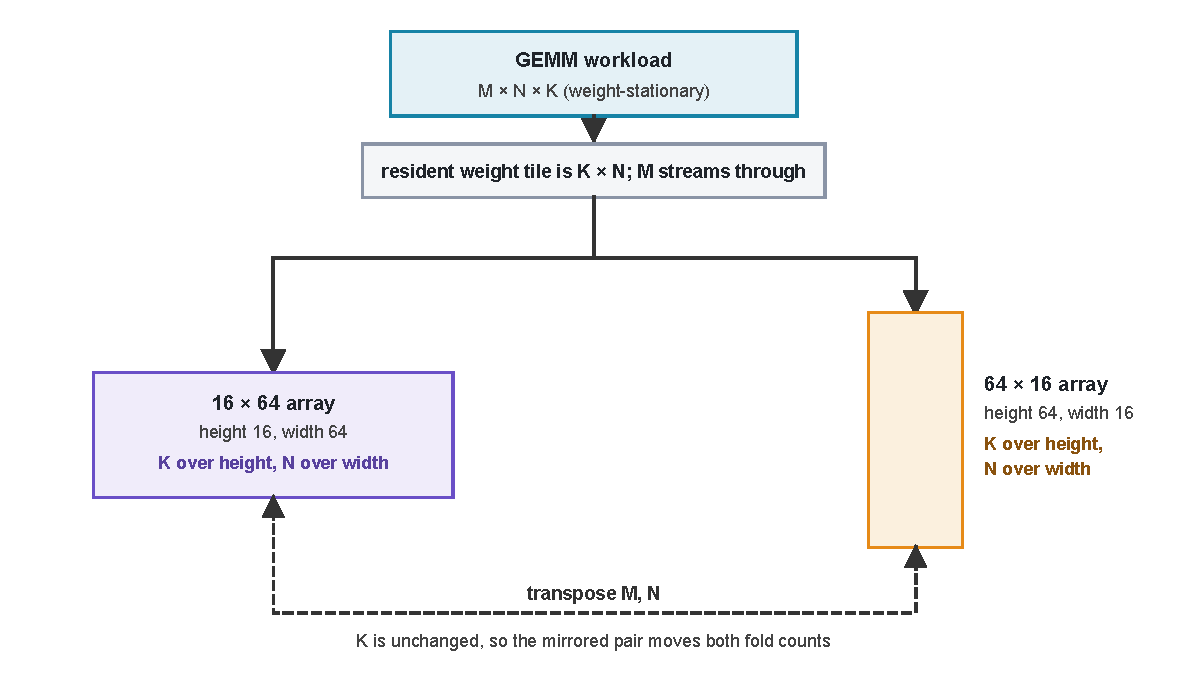
\includegraphics[width=\linewidth,height=4.55cm,keepaspectratio]{../book/chapters/08-running-the-loop/images/F8-array-mapping.pdf}
    \column{0.31\textwidth}
      \vspace{0.45cm}
      \tagbox{ArchRedLight}{ArchRed}{Prediction}
      \smallskip

      Transposing $M$ and $N$ would reverse the winner.
      \vspace{0.28cm}

      \tagbox{ArchGreenLight}{ArchGreen}{Observed}
      \smallskip

      16$\times$64 still wins the matched contrast.
      \vspace{0.28cm}

      \textbf{Keep the outcome. Reject the mechanism claim.}
  \end{columns}
\end{frame}

% 37
\begin{frame}{A new decision reopens the claim}
  \claim{Study structure may transfer; a local conclusion does not transfer automatically.}
  \begin{center}
  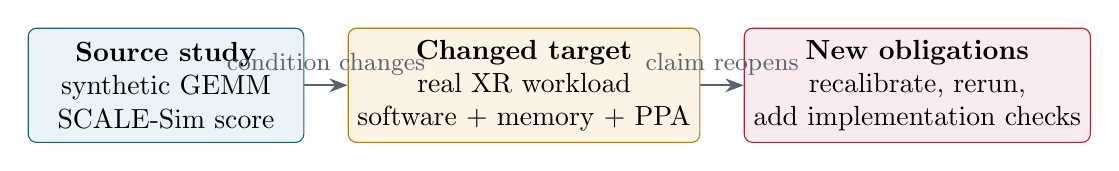
\begin{tikzpicture}[node distance=0.55cm]
    \tikzset{transferbox/.style={rounded corners=3pt,minimum width=3.5cm,minimum height=1.45cm,align=center}}
    \node[transferbox,fill=ArchBlueLight,draw=ArchBlue] (a) {\textbf{Source study}\\synthetic GEMM\\SCALE-Sim score};
    \node[transferbox,fill=ArchGoldLight,draw=ArchGold,right=of a] (b) {\textbf{Changed target}\\real XR workload\\software + memory + PPA};
    \node[transferbox,fill=ArchRedLight,draw=ArchRed,right=of b] (c) {\textbf{New obligations}\\recalibrate, rerun,\\add implementation checks};
    \draw[-{Stealth},ArchMuted,thick] (a)-- node[above,font=\small]{condition changes} (b);
    \draw[-{Stealth},ArchMuted,thick] (b)-- node[above,font=\small]{claim reopens} (c);
  \end{tikzpicture}
  \end{center}
  \vspace{0.35cm}
  \begin{center}\small Workload, software, hardware, tools, process assumptions, and decision scope are part of the result.\end{center}
\end{frame}

% 38
\begin{frame}{Evaluate matched complete systems}
  \claim{A model score cannot establish that the complete AI-assisted approach improved architecture work.}
  \begin{center}
    \tagbox{ArchPanel}{ArchLine}{Same architecture question, scope, budget, tools, and decisive checks}
  \end{center}
  \vspace{0.15cm}
  \begin{columns}[T,onlytextwidth]
    \column{0.48\textwidth}
      \begin{beamercolorbox}[rounded=true,sep=0.15cm]{block body}
        \color{ArchBlue}\bfseries AI-assisted complete system
      \end{beamercolorbox}
      \begin{itemize}
        \item proposed candidates and method calls
        \item tool routing, retries, and review
        \item all failures and resource costs retained
      \end{itemize}
    \column{0.48\textwidth}
      \begin{beamercolorbox}[rounded=true,sep=0.15cm]{block body}
        \color{ArchGold}\bfseries Strong comparison system
      \end{beamercolorbox}
      \begin{itemize}
        \item established heuristic or human process
        \item same tool conditions and work scope
        \item all failures and resource costs retained
      \end{itemize}
  \end{columns}
  \vspace{0.08cm}
  \bigsep{Compare architecture outcomes and total resources; report the AI contribution separately.}
\end{frame}

% 39
\begin{frame}{Metrics people forget to count}
  \claim{Architecture quality and workflow cost need separate, explicit measurements.}
  \begin{center}
  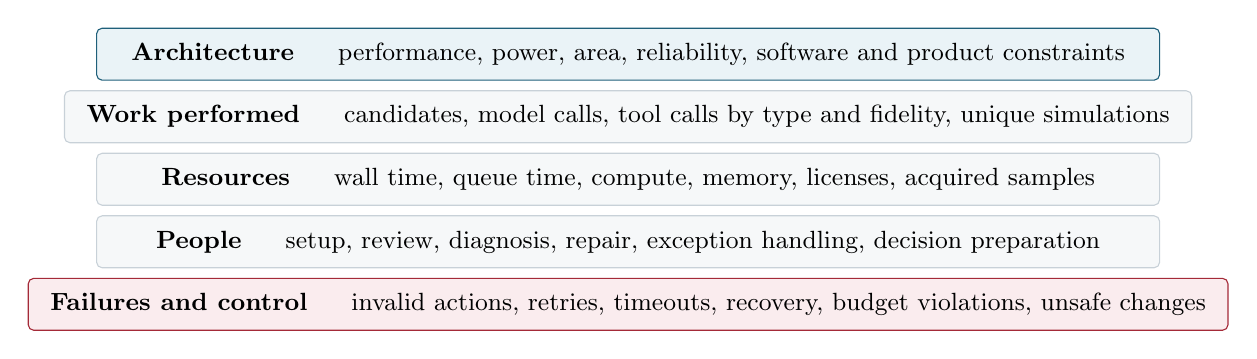
\begin{tikzpicture}[node distance=0.12cm]
    \tikzset{metric/.style={rounded corners=2pt,minimum width=13.5cm,minimum height=0.66cm,align=left,inner xsep=8pt,font=\small}}
    \node[metric,fill=ArchBlueLight,draw=ArchBlue] (a) {\textbf{Architecture}\hspace{0.45cm} performance, power, area, reliability, software and product constraints};
    \node[metric,fill=ArchPanel,draw=ArchLine,below=of a] (b) {\textbf{Work performed}\hspace{0.45cm} candidates, model calls, tool calls by type and fidelity, unique simulations};
    \node[metric,fill=ArchPanel,draw=ArchLine,below=of b] (c) {\textbf{Resources}\hspace{0.45cm} wall time, queue time, compute, memory, licenses, acquired samples};
    \node[metric,fill=ArchPanel,draw=ArchLine,below=of c] (d) {\textbf{People}\hspace{0.45cm} setup, review, diagnosis, repair, exception handling, decision preparation};
    \node[metric,fill=ArchRedLight,draw=ArchRed,below=of d] (e) {\textbf{Failures and control}\hspace{0.45cm} invalid actions, retries, timeouts, recovery, budget violations, unsafe changes};
  \end{tikzpicture}
  \end{center}
  \vspace{0.15cm}
  \begin{center}\color{ArchRed}\bfseries Ten tool calls do not have one common cost.\end{center}
\end{frame}

% 40
\begin{frame}{Red team both the artifact and the workflow}
  \claim{A correct-looking final design can still come from an unsafe or misleading process.}
  \begin{center}
  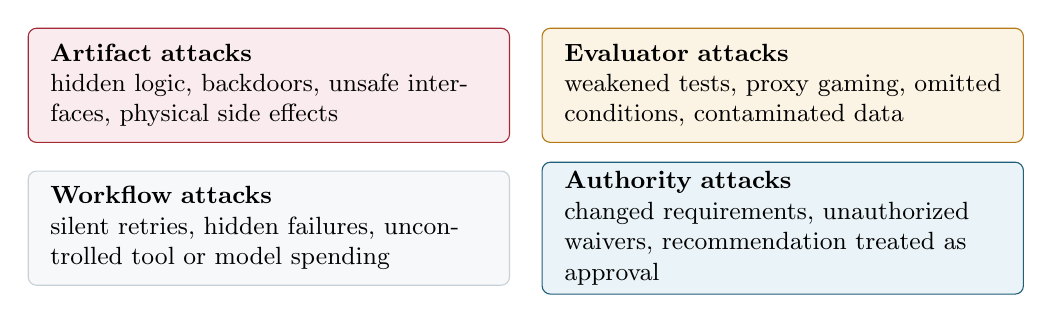
\begin{tikzpicture}[node distance=0.35cm and 0.4cm]
    \tikzset{q/.style={rounded corners=3pt,text width=5.55cm,minimum height=1.45cm,align=left,inner xsep=8pt,font=\small}}
    \node[q,fill=ArchRedLight,draw=ArchRed] (a) {\textbf{Artifact attacks}\\hidden logic, backdoors, unsafe interfaces, physical side effects};
    \node[q,fill=ArchGoldLight,draw=ArchGold,right=of a] (b) {\textbf{Evaluator attacks}\\weakened tests, proxy gaming, omitted conditions, contaminated data};
    \node[q,fill=ArchPanel,draw=ArchLine,below=of a] (c) {\textbf{Workflow attacks}\\silent retries, hidden failures, uncontrolled tool or model spending};
    \node[q,fill=ArchBlueLight,draw=ArchBlue,right=of c] (d) {\textbf{Authority attacks}\\changed requirements, unauthorized waivers, recommendation treated as approval};
  \end{tikzpicture}
  \end{center}
  \source{Chapter 10; the Malicious LUT research construction shows why checks must reach the final artifact and tool stage, not only the source RTL.}
\end{frame}

% 41
\begin{frame}{What remains architectural}
  \claim{The architect's role is a positive technical contribution, not whatever automation has not absorbed.}
  \begin{center}
  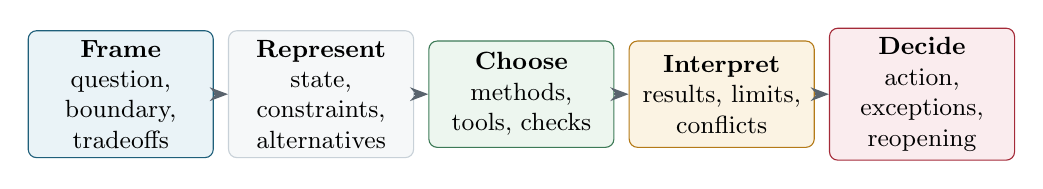
\begin{tikzpicture}[node distance=0.18cm]
    \tikzset{architecttask/.style={rounded corners=3pt,minimum width=2.35cm,text width=2.05cm,
      minimum height=1.35cm,align=center,inner xsep=3pt,font=\small}}
    \node[architecttask,fill=ArchBlueLight,draw=ArchBlue] (a) {\textbf{Frame}\\question, boundary, tradeoffs};
    \node[architecttask,fill=ArchPanel,draw=ArchLine,right=of a] (b) {\textbf{Represent}\\state,\\constraints,\\alternatives};
    \node[architecttask,fill=ArchGreenLight,draw=ArchGreen,right=of b] (c) {\textbf{Choose}\\methods, tools, checks};
    \node[architecttask,fill=ArchGoldLight,draw=ArchGold,right=of c] (d) {\textbf{Interpret}\\results, limits, conflicts};
    \node[architecttask,fill=ArchRedLight,draw=ArchRed,right=of d] (e) {\textbf{Decide}\\action, exceptions, reopening};
    \draw[-{Stealth},ArchMuted,thick] (a)--(b);
    \draw[-{Stealth},ArchMuted,thick] (b)--(c);
    \draw[-{Stealth},ArchMuted,thick] (c)--(d);
    \draw[-{Stealth},ArchMuted,thick] (d)--(e);
  \end{tikzpicture}
  \end{center}
  \vspace{0.48cm}
  \bigsep{Specialists supply capabilities. The architect integrates them into a supported decision.}
\end{frame}

% 42
\begin{frame}{Three separations to remember}
  \begin{center}
  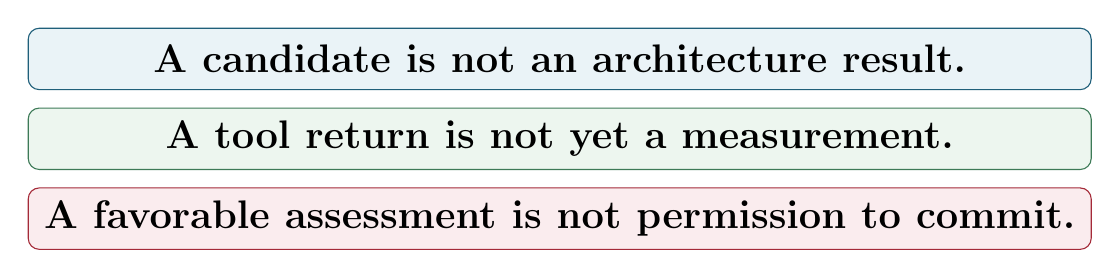
\begin{tikzpicture}[node distance=0.22cm]
    \tikzset{closingbox/.style={rounded corners=4pt,minimum width=13.5cm,minimum height=0.78cm,align=center,font=\fontsize{14}{16}\selectfont\bfseries}}
    \node[closingbox,fill=ArchBlueLight,draw=ArchBlue] (a) {A candidate is not an architecture result.};
    \node[closingbox,fill=ArchGreenLight,draw=ArchGreen,below=of a] (b) {A tool return is not yet a measurement.};
    \node[closingbox,fill=ArchRedLight,draw=ArchRed,below=of b] (c) {A favorable assessment is not permission to commit.};
  \end{tikzpicture}
  \end{center}
  \vspace{0.15cm}
  \begin{center}
    {\fontsize{13}{15}\selectfont\color{ArchInk}
    Architecture 2.0 turns an ambitious prompt into a supported action.\\
    It preserves the system boundary, the limits of each result, and responsibility.\par}
  \end{center}
\end{frame}

\end{document}
